%!TEX TS-program = xelatex
\documentclass[12pt,a4paper, oneside]{extreport}

%%%%%%%%%% Математика %%%%%%%%%%
\usepackage{amsmath,amsfonts,amssymb,amsthm,mathtools}
% Показывать номера только у тех формул, на которые есть \eqref{} в тексте.
%\mathtoolsset{showonlyrefs=true}
%\usepackage{leqno} % Нумерация формул слева
%\usepackage{tipa} %Для формулки из логитов


% \noindent
% уравнение ()

\usepackage{hyphenat}


%%%%%%%%%% Шрифты %%%%%%%%
\usepackage[english, russian]{babel} % выбор языка для документа
\usepackage[utf8]{inputenc} % задание utf8 кодировки исходного tex файла
\usepackage[X2,T2A]{fontenc}        % кодировка

\usepackage{fontspec}         % пакет для подгрузки шрифтов
\setmainfont{Times New Roman}       % задаёт основной шрифт документа

\usepackage{unicode-math}      % пакет для установки математического шрифта
\setmathfont{Asana-Math.otf}    % шрифт для математики

% Конкретный символ из конкретного шрифта
% \setmathfont[range=\int]{Neo Euler}




%%%%%%%%%% Работа с картинками %%%%%%%%%
\usepackage{graphicx}                  % Для вставки рисунков
\usepackage{graphics}
\graphicspath{{images/}{pictures/}}    % можно указать папки с картинками
\usepackage{wrapfig}                   % Обтекание рисунков и таблиц текстом


%%%%%%%%%% Работа с таблицами %%%%%%%%%%
\usepackage{tabularx}            % новые типы колонок
\usepackage{tabulary}            % и ещё новые типы колонок
\usepackage{array,delarray}      % Дополнительная работа с таблицами
\usepackage{longtable}           % Длинные таблицы
\usepackage{multirow}            % Слияние строк в таблице
\usepackage{float}               % возможность позиционировать объекты в нужном месте

\usepackage{booktabs}            % таблицы как в книгах
% Заповеди из документации к booktabs:
% 1. Будь проще! Глазам должно быть комфортно
% 2. Не используйте вертикальные линни
% 3. Не используйте двойные линии. Как правило, достаточно трёх горизонтальных линий
% 4. Единицы измерения - в шапку таблицы
% 5. Не сокращайте .1 вместо 0.1
% 6. Повторяющееся значение повторяйте, а не говорите "то же"
% 7. Есть сомнения? Выравнивай по левому краю!

%  вычисляемые колонки по tabularx
\newcolumntype{C}{>{\centering\arraybackslash}X}
\newcolumntype{L}{>{\raggedright\arraybackslash}X}
\newcolumntype{Y}{>{\arraybackslash}X}
\newcolumntype{Z}{>{\centering\arraybackslash}X}


%%%%%%%%%% Графика и рисование %%%%%%%%%%
\usepackage{tikz, pgfplots}      % язык для рисования графики из latex'a

%%%%%%%%%% Гиперссылки %%%%%%%%%%
\usepackage{xcolor}              % разные цвета

\usepackage{hyperref}
\hypersetup{
	unicode=true,           % позволяет использовать юникодные символы
	colorlinks=true,       	% true - цветные ссылки, false - ссылки в рамках
	urlcolor =blue,         % цвет ссылки на url
	linkcolor=black,        % внутренние ссылки
	citecolor=black,        % на библиографию
	breaklinks              % если ссылка не умещается в одну строку, разбивать ли ее на две части?
}


%%%%%%%%%% Другие приятные пакеты %%%%%%%%%
\usepackage{multicol}       % несколько колонок
\usepackage{verbatim}       % для многострочных комментариев
\usepackage{cmap} % для кодировки шрифтов в pdf

\usepackage{enumitem} % дополнительные плюшки для списков
%  например \begin{enumerate}[resume] позволяет продолжить нумерацию в новом списке

\usepackage{todonotes} % для вставки в документ заметок о том, что  осталось сделать
% \todo{Здесь надо коэффициенты исправить}
% \missingfigure{Здесь будет Последний день Помпеи}
% \listoftodos --- печатает все поставленные \todo'шки




\usepackage[bottom]{footmisc}

%%%%%%%%%%%%%% ГОСТОВСКИЕ ПРИБАМБАСЫ %%%%%%%%%%%%%%%

%%% размер листа бумаги
\usepackage[paper=a4paper,top=15mm, bottom=15mm,left=35mm,right=10mm,includehead]{geometry}


\usepackage{setspace}
\setstretch{1.33}     % Межстрочный интервал
\setlength{\parindent}{1.25cm} % Красная строка.


%\flushbottom       % Эта команда заставляет LaTeX чуть растягивать строки, чтобы получить идеально прямоугольную страницу
\righthyphenmin=2  % Разрешение переноса двух и более символов
\widowpenalty=10000  % Наказание за вдовствующую строку (одна строка абзаца на этой странице, остальное --- на следующей)
%\clubpenalty=10000  % Наказание за сиротствующую строку (омерзительно висящая одинокая строка в начале страницы)
\tolerance=1000     % Ещё какое-то наказание.


% Нумерация страниц сверху по центру
\usepackage{fancyhdr}
\pagestyle{fancy}
\fancyhead{ } % clear all fields
\fancyfoot{ } % clear all fields
\fancyhead[C]{\thepage}
% Чтобы не прорисовывалась черта!
\renewcommand{\headrulewidth}{0pt}


% Нумерация страниц с надписью "Глава"
\usepackage{etoolbox}
\patchcmd{\chapter}{\thispagestyle{plain}}{\thispagestyle{fancy}}{}{}


%%% Заголовки
\usepackage[indentfirst]{titlesec}{\raggedleft}
% Заголовки по левому краю
% опция identfirst устанавливает отступ в первом абзаце



% В Linux этот пакет сделан косячно. Исправляет это следующий непонятный кусок кода.
\makeatletter
\patchcmd{\ttlh@hang}{\parindent\z@}{\parindent\z@\leavevmode}{}{}
\patchcmd{\ttlh@hang}{\noindent}{}{}{}
\makeatother


% Редактирования Глав и названий
\titleformat{\chapter}
{\normalfont\large\bfseries}
{\thechapter }{0.5 em}{}

% Редактирование ненумеруемых глав chapter* (Введение и тп)
\titleformat{name=\chapter,numberless}
{\centering\normalfont\bfseries\large}{}{0.25em}{}

% Убирает чеканутые отступы вверху страницы
\titlespacing{\chapter}{0pt}{-\baselineskip}{\baselineskip}

% Более низкие уровни
\titleformat{\section}{\bfseries}{\thesection}{0.5 em}{}
\titleformat{\subsection}{\bfseries}{\thesubsection}{0.5 em}{}

\titlespacing*{\section}{0 pt}{\baselineskip}{\baselineskip}
\titlespacing*{\subsection}{0 pt}{\baselineskip}{\baselineskip}


% Содержание. Команды ниже изменяют отступы и рисуют точечки!
\usepackage{titletoc}

\titlecontents{chapter}
[1em] %
{\normalsize}
{\contentslabel{1 em}}
{\hspace{-1 em}}
{\normalsize\titlerule*[10pt]{.}\contentspage}

\titlecontents{section}
[3 em] %
{\normalsize}
{\contentslabel{1.75 em}}
{\hspace{-1.75 em}}
{\normalsize\titlerule*[10pt]{.}\contentspage}

\titlecontents{subsection}
[6 em] %
{\normalsize}
{\contentslabel{3 em}}
{\hspace{-3 em}}
{\normalsize\titlerule*[10pt]{.}\contentspage}


% Правильные подписи под таблицей и рисунком
% Документация к пакету на русском языке!
\usepackage[tableposition=top, singlelinecheck=false]{caption}
\usepackage{subcaption}


\DeclareCaptionStyle{base}%
[justification=centering,indention=0pt]{}
\DeclareCaptionLabelFormat{gostfigure}{Рисунок #2}
\DeclareCaptionLabelFormat{gosttable}{Таблица #2}

\DeclareCaptionLabelSeparator{gost}{~---~}
\captionsetup{labelsep=gost}

\DeclareCaptionStyle{fig01}%
[margin=5mm,justification=centering]%
{margin={3em,3em}}
\captionsetup*[figure]{style=fig01,labelsep=gost,labelformat=gostfigure,format=hang}

\DeclareCaptionStyle{tab01}%
[margin=5mm,justification=centering]%
{margin={3em,3em}}
\captionsetup*[table]{style=tab01,labelsep=gost,labelformat=gosttable,format=hang}


% межстрочный отступ в таблице
\renewcommand{\arraystretch}{1.2}



% многостраничные таблицы под РОССИЙСКИЙ СТАНДАРТ
% ВНИМАНИЕ! Обязательно за CAPTION !
\usepackage{fr-longtable}



%Более гибкие спсики
\usepackage{enumitem}
% сообщаем окружению о том, что существует такая штук как нумерация русскими буквами.
\makeatletter
\AddEnumerateCounter{\asbuk}{\russian@alph}{щ}
\makeatother


%%% ГОСТОВСКИЕ СПИСКИ

% Первый тип списков. Большая буква.
\newlist{Enumerate}{enumerate}{1}

\setlist[Enumerate,1]{labelsep=0.5em,leftmargin=1.25em,labelwidth=1.25em,
	parsep=0em,itemsep=0em,topsep=0ex, before={\parskip=-1em},label=\arabic{Enumeratei}.}



% Второй тип списков. Маленькая буква.
\setlist[enumerate]{label=\arabic{enumi}),parsep=0em,itemsep=0em,topsep=0.75ex, before={\parskip=-1em}, leftmargin = 2.76em}



% Третий тип списков. Два уровня.
\newlist{twoenumerate}{enumerate}{2}
\setlist[twoenumerate,1]{itemsep=0mm,parsep=0em,topsep=0.75ex,, before={\parskip=-1em},label=\asbuk{twoenumeratei})}
\setlist[twoenumerate,2]{leftmargin=1.3em,itemsep=0mm,parsep=0em,topsep=0ex, before={\parskip=-1em},label=\arabic{twoenumerateii})}


% Четвёртый тип списков. Список с тире.
\setlist[itemize]{label=--,parsep=0em,itemsep=0em,topsep=0ex, before={\parskip=-1em},after={\parskip=-1em}}


%%% WARNING WARNING WARNIN!
%%% Если в списке предложения, то должна по госту стоять точка после цифры => команда Enumerate! Если идет перечень маленьких фактов, не обособляемых предложений то после цифры идет скобка ")" => команда enumerate! Если перечень при этом ещё и двууровневый, то twoenumerate.




%%%%%%%%%% Список литературы %%%%%%%%%%

%\usepackage[%
%backend=biber, %подключение пакета biber (тоже нужен)
%bibstyle=gost-numeric, %подключение одного из четырех главных стилей biblatex-gost
%sorting=ntvy, %тип сортировки в библиографии
%]{biblatex}
\usepackage[backend=biber,style=gost-numeric, maxbibnames=9,maxcitenames=2,uniquelist=false, babel=other]{biblatex}



% Справка по 4 главным стилям для ленивых:
% gost-inline  ссылки внутри теста в круглых скобках
% gost-footnote подстрочные ссылки
% gost-numeric затекстовые ссылки
% gost-authoryear тоже затекстовые ссылки, но немного другие

% Подробнее смотри страницу 4 документации. Она на русском.

% Ещё немного настроек
\DeclareFieldFormat{postnote}{#1} %убирает с. и p.
\renewcommand*{\mkgostheading}[1]{#1} % только лишь убираем курсив с авторов


\addbibresource{diplomabib.bib} % сюда нужно вписать свой bib-файлик.

% Этот кусок кода выносит русские источники на первое место. Костыль описали авторы пакета в руководстве к нему. Подробнее смотри:
% https://github.com/odomanov/biblatex-gost/wiki/Как-сделать%2C-чтобы-русскоязычные-источники-предшествовали-остальным
\DeclareSourcemap{
	\maps[datatype=bibtex]{
		\map{
			\step[fieldsource=langid, match=russian, final]
			\step[fieldset=presort, fieldvalue={a}]
		}
		\map{
			\step[fieldsource=langid, notmatch=russian, final]
			\step[fieldset=presort, fieldvalue={z}]
		}
	}
}

\DefineBibliographyStrings{english}{%
	pages = {P\adddot},
	number = {№},
}


\begin{document} % Начала документа

\thispagestyle{empty} % Чтобы избежать нумерации титульника

% Если для какой-то страницы хочется сделать своё уникальное оформление, как например для титульника или списка литературы, то можно использовать окружение \begingroup ... \endgroup. 
\begingroup
\setstretch{1}   % Убираем полторашные интервалы на титульнике
\begin{center}
\small \bfseries Федеральное государственное бюджетное образовательное учреждение высшего образования

<<РОССИЙСКАЯ АКАДЕМИЯ НАРОДНОГО ХОЗЯЙСТВА и\\ ГОСУДАРСТВЕННОЙ СЛУЖБЫ \\
при Президенте Российской Федерации>>

\vspace{2ex}

\bfseries
ИНСТИТУТ ЭКОНОМИКИ, МАТЕМАТИКИ И ИНФОРМАЦИОННЫХ\\ ТЕХНОЛОГИЙ

ЭКОНОМИЧЕСКИЙ ФАКУЛЬТЕТ

НАПРАВЛЕНИЕ 38.03.01 ЭКОНОМИКА
\end{center}

\vfill


\noindent  Группа ЭО-15-01
\hfill
\parbox[t]{20em}{\centering
Кафедра микроэкономики

\mbox{ }

\textbf{Допустить к защите}

заведующий кафедрой микроэкономики

\mbox{ }

\rule{8em}{0.5pt} М.И. Левин

\mbox{ }

<<\rule{2em}{0.5pt}>> \rule{5em}{0.5pt} 201\rule{1em}{0.5pt} г. }

\mbox{ }

\mbox{ }

\begin{center}\bfseries
ВЫПУСКНАЯ КВАЛИФИКАЦИОННАЯ РАБОТА

\mbox{ }

\large
ПРОГНОЗИРОВАНИЕ   \\
ИЕРАРХИЧЕСКИХ ВРЕМЕННЫХ РЯДОВ
\end{center}

\vfill

\noindent\normalsize
студент-бакалавр

\noindent
Касьянова Ксения Алексеевна
\hfill /\rule{6em}{0.5pt}/\rule{6em}{0.5pt}/

\hfill\makebox[13em]{\hfill\footnotesize (подпись) \hfill\hfill (дата) \hfill}

\noindent
научный руководитель выпускной \\
квалификационной работы

\noindent
ст. преп. Демешев Борис Борисович
\hfill /\rule{6em}{0.5pt}/\rule{6em}{0.5pt}/

\hfill\makebox[13em]{\hfill\footnotesize (подпись) \hfill\hfill (дата) \hfill}

%\noindent
%консультант
%
%\noindent
%д.э.н., профессор Петров Петр Петрович
%\hfill /\rule{6em}{0.5pt}/\rule{6em}{0.5pt}/
%
%\hfill\makebox[13em]{\hfill\footnotesize (подпись) \hfill\hfill (дата) \hfill}

\vfill

\begin{center}
\normalsize \bfseries МОСКВА \\ 2019 г.
\end{center}
\endgroup



%%%%%%%%%%%%%%%%%%% ОГЛАВЛЕНИЕ %%%%%%%%%%%%%%%%%%%%%%%%%%%%%%%%%%%%%%

\tableofcontents  % Команда, которая создаёт оглавление


%%%%%%% ВВЕДЕНИЕ %%%%%%

\chapter*{Введение}
%Включение введения в соодержание
\addcontentsline{toc}{chapter}{Введение}


В анализе данных часто встречаются данные со сложной многоуровневой структурой, точный прогноз которых является одним из ключевых факторов принятия эффективных решений. 
Необходимость прогнозирования данных с иерархической структурой возникает, например, в микроэкономике при анализе спроса, макроэкономике, страховании,  демографии и т.д. 
%В связи с этим необходимо использовать  подходы, позволяющие учитывать взаимозависимости прогнозируемых временных рядов.  


В данной работе исследуются методы прогнозирования иерархических временных рядов, учитывающие зависимость между уровнями агрегирования и внутри одного уровня. 
%Теоретической основой исследования послужили работы ученых в области анализа данных, прогнозирования и моделирования.
Цель работы: сравнение моделей, учитывающих иерархическую структуру данных, выявление факторов, позволяющих улучшить прогнозы агрегированного временного ряда.
Достижение поставленной цели предполагает постановку и решение следующих задач:

%используя модели, учитывающие иерархическую структуру данных, улучшить прогнозы агрегированного временного ряда.

%использовать информацию на одном уровне агрегирования для улучшения прогнозов на другом уровне агрегирования. 


\begin{itemize}
	\item сбор данных с трехуровневой иерархической структурой;
	\item выбор моделей для прогнозирования агрегированного ряда;
%	\item сравнение ARIMA моделей с использованием дополнительных регрессоров (ближайшего по метрике корреляции временного ряда третьего уровня, ряда второго уровня или прогноза ряда второго уровня) и без;    
	\item сравнение различных методов комбинирования прогнозов нижних рядов, полученных по выбранным моделям; 
	\item сравнение качества прогнозов полученным по рядам второго уровня, сгруппированным по оригинальным  (по территориальному признаку и по классу) и полученным с помощью кластеризации признакам;
	\item прогнозирование рядов второго и третьего уровня по выбранным моделям, сравнение суммы и оптимальной комбинации этих прогнозов с прогнозом агрегированного временного ряда.
%	\item сравнение прогнозной силы моделей для агрегированного временного ряда, взвешенных прогнозов дизагрегированных рядов; % и иерархической байесовской модели.
%\item  Добавление в модель дамми структурного сдвига






%Visualizing data and coeffictent distributions


%Writing CV code


%Developing a detailed scoring mechanism to rank attributes and record the process of ranking will always be useful.


\end{itemize}


%Актуальность
%Методы, описанные в данной работе актуальны при необходимости прогнозирования, как агрегированного ряда, так и отдельных компонент, составляющих его, а также получения подтверждения правильности выбора модели для агрегированного ряда.
%Для анализа были выбраны ряды с определенной структурой, а именно: 
%структура трехуровневая и иерархическая, причем сам агрегированный ряд и ряды второго уровня можно получить при суммировании рядов третьего уровня. 
%В ходе исследования мы определим,  позволяет ли такое детальное дробление временного ряда на более мелкие добиться существенного улучшения прогнозов или можно, например, ограничиться двумя уровнями.


% теоретическую и практическую значимость работы (если работа претендует на значи-мые результаты в этих аспектах)

Применение иерархических моделей на трех наборах данных, обладающих различными характеристиками,    с использованием кросс-валидации со скользящим окном позволяет получить более устойчивые  выводы. 





Данная работа состоит из введения, двух глав основной части, заключения и приложений. В первой главе рассматриваются основные модели прогнозирования иерархических временных рядов.  Во второй главе проводится  сравнение моделей применительно к собранным данным с требуемой структурой. 
В приложении (А) содержатся коды для выгрузки данных. В приложении (\ref{app-a}) содержатся графики, отражающие многоуровневую структуру данных. В приложении (\ref{app-b}) представлены таблицы, позволяющие сравнить качество прогнозов, полученное по различным моделям. 




% степень ее разработанности


%методологию и методы исследования;

%положения, выносимые на защиту;



\chapter{Модели \ \ прогнозирования \ \ временных рядов \ \   с \ \ иерархической \\ структурой}



\section{Обзор литературы}


%С    развитием различных социально-экономических процессов, укрепляется и взаимосвязь между ними. 


В современной  литературе по анализу данных можно выделить несколько основных подходов к  прогнозированию временных рядов с иерархической структурой. 
Основное предположение, на котором построены многие из методов, заключается в том, что при группировке  рядов, которые ведут себя одинаково, характерные ошибки внутри групп будут  компенсировать друг друга, в то время как более релевантная для прогнозирования  индивидуальная динамика будет сохраняться.

Одним из способов повышения точности прогнозов является агрегирование данных до составления прогнозов, другой -- комбинирование  самих прогнозов. 
Информация полученная из агрегированных рядов может иметь существенное влияние при прогнозировании рядов нижнего уровня, хотя ее использование может сопровождаться некоторыми сложностями, возникающих из-за индивидуальных особенностей рядов. 



Принципиально другим методом работы с иерархическими временным рядами явлется байесовский подход. Для рядов относящихся к одной группе подбирается одинаковое априорное распределение коэффициентов.
В простых случаях  эффект от выбора такого априорного распределения  такой: если ряды сильно отчаются от сгруппированных, то влияние группового априорного распределения уменьшается,  апостериорное распределение коэффициентов для них сужается.
%Однако, если при  изменении одного априорного распределения на другое разумное ответы значительно изменятся, то необходимо собрать больше данных.

%Одной из наиболее распространенных моделей прогнозирования взаимозависимых рядов является модель векторной авторегрессии (VAR), однако ее использование может сопровождаться некоторыми сложностями, например, при большое число лагов в модели приводит значительному росту числа оцениваемых коэффициентов.  


Альтернативными моделями, подходящими для прогнозирования  временных рядов с многоуровневой  структурой являются, например, модель  векторной авторегрессии (VAR), в которой  временные ряды, относящиеся к одной группе, могут  иметь общие параметры. В качестве некой альтернативы этому методу можно предложить использование модели ARIMA с дополнительными регрессорами, полученными из прогнозируемого набора данных. 

Для прогнозирования иерархических рядов в том числе применяются многомерные модели пространства состояний, векторное  экспоненциальное сглаживание, а также  байесовские подходы применительно  к пулу аналогичных временных рядов\cite{duncan2001forecasting}.
Эмпирические результаты показали, что с помощью перечисленных выше методов точность прогноза может быть улучшена, поскольку при оценке параметров учитывается    зависимость  между временными рядами, принадлежащими одной группе. Однако использование этих моделей связано с выполнением большого числа предпосылок или введения соответствующих ограничений.


Во многих теоретических и эмпирических работах было замечено, что зачастую более простые методы  оказываются в разы эффективнее, сложных моделей с большим числом оцениваемых  коэффициентов. 
Такой    подход к прогнозированию рядов, как получение оптимальной комбинации прогнозов  по качеству прогнозов может легко обогнать модели, учитывающие особенности каждого из рядов при оценивании коэффициентов. 




%
%\textbf{Shrinkage} is implicit in Bayesian inference and penalized likelihood inference, and explicit in James–Stein-type inference. In contrast, simple types of maximum-likelihood and least-squares estimation procedures do not include shrinkage effects, although they can be used within shrinkage estimation schemes.
%
%
%\textbf{Stein's  paradox}, in decision theory and estimation theory, is the phenomenon that when three or more parameters are estimated simultaneously, there exist combined estimators more accurate on average (that is, having lower expected mean squared error) than any method that handles the parameters separately. 
%
%\textit{The best guess about the future is usually  obtained by computing the average of past events. Stein's paradox defines circumstances in which there are estimators better that the arithmetic average
%}
%
%Stein’s paradox  **modern generalization, the Bayesian hierarchical model**. 
%
%Bayesian hierarchical model can improve overall estimation accuracy, thereby improving our confidence in the assessment results, especially for standard compliance assessment of waters with **small sample sizes.**
%

\section{Комбинирование прогнозов}

Существует несколько   популярных     подходов к комбинированию прогнозов:   «сверху-вниз», «снизу-вверх», <<из середины>> и корректировка прогнозов по OLS. 
Данные, к которым эти подходы  применимы, отличаются следующим свойством: 
когда ряды нижнего уровня  группируются, прогнозы каждой группы должны быть равны сумме прогнозов рядов, входящих в  группу.

Для любого набора данных, обладающего  таким свойством можно построить суммирующую матрицу $S$, которая отражает  структуру иерархии рядов. 
Примером такой матрицы является:

\begin{equation}\label{key123}
\begin{bmatrix}
y_{t} \\
y_{1, t} \\
y_{2, t} \\
... \\
y_{i, t} \\
y_{11, t} \\
y_{12, t} \\
y_{13, t} \\
y_{21, t} \\
y_{22, t} \\
y_{23, t} \\

... \\
y_{ij-2, t} \\
y_{ij-1, t} \\
y_{ij, t}
\end{bmatrix}
=
\begin{bmatrix}
1& 1 &1& 1& 1& 1& ... &1& 1& 1 \\
1 &1& 1& 0& 0& 0& ... &0 &0 &0  \\
0 &0 &0 &1& 1& 1& ... &0 &0 &0  \\
0& 0& 0& 0& 0& 0& ...&0 &0 &0 \\ 
0& 0& 0& 0& 0& 0& ...& 1& 1& 1 \\
1 &0 &0& 0& 0& 0& ...& 0& 0& 0 \\
0 &1 &0& 0& 0& 0& ...& 0& 0& 0 \\
0 &0 &1& 0& 0& 0& ...& 0& 0& 0 \\
0 &0 &0& 1& 0& 0& ...& 0& 0& 0 \\
0 &0 &0& 0& 1& 0& ...& 0& 0& 0 \\
0 &0 &0& 0& 0& 1& ...& 0& 0& 0 \\
0& 0& 0& 0& 0& 0& ...&0 &0 &0  \\ 
0 &0 &0& 0& 0& 0& ...& 1& 0& 0 \\
0 &0 &0& 0& 0& 0& ...& 0& 1& 0 \\
0 &0 &0& 0& 0& 0& ...& 0& 0& 1 
\end{bmatrix}
\begin{bmatrix}
y_{11, t} \\
y_{12, t} \\
y_{13, t} \\
y_{21, t} \\
y_{22, t} \\
y_{23, t} \\

... \\
y_{ij-2, t} \\
y_{ij-1, t} \\
y_{ij, t}
\end{bmatrix},
\end{equation}

\noindent
где $y_{ij,t}, y_{i,t},  y_{t}  $ -- значения $j$-ого ряда третьего уровня, $i$-ого ряда второго уровня и ряда первого уровня соответственно в момент времени $t$. Схематически такая  структура данных представлена на рисунке (\ref{fig:screenshot51}). 

\newpage

\begin{figure}
	\centering
	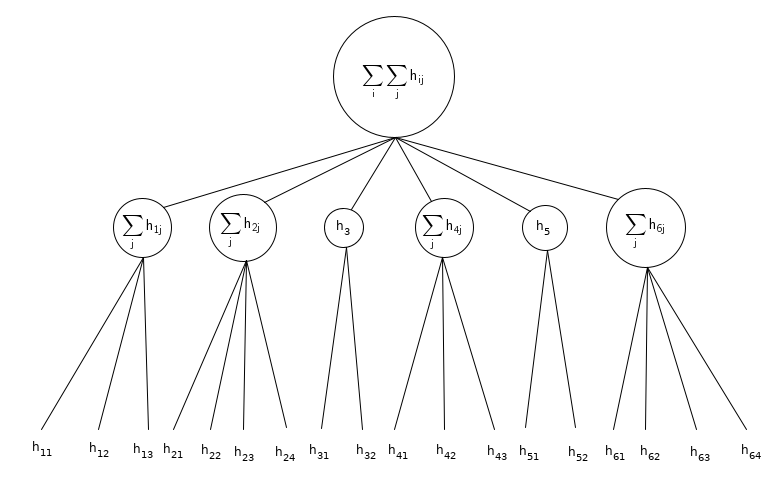
\includegraphics[width=0.7\linewidth]{Screenshot51}
	\caption{Структура временных рядов, необходимых для исследования}
	\label{fig:screenshot51}
	

\end{figure}




Переписав уравнение (\ref{key123})  в более компактной форме имеем: 

\begin{equation}\label{key}
y_t  = S b_t ,
\end{equation}

\noindent
где $y_t$ -- вектор размерности $(n \times 1)$ всех наблюдений на всех уровнях иерархии в момент времени $t$, $ n = 1+i+\sum_i j$, $S$  -- суммирующая матрица, отражающая иерархическую структуру данных,  
$ b_t $ -- вектор размерности $(m \times 1)$ всех наблюдений на самом нижнем уровне иерархии в момент времени $t$, $ m =\sum_i j$ 


\subsection{Метод <<снизу-вверх>>}


Самый распространенный метод получения прогнозов для всех уровней иерархии --  <<снизу-вверх>> метод (англ. bottom-up). Суть метода заключается в получении независимых прогнозов на $h$ шагов вперед  для рядов нижнего уровня иерархии  и  их агрегирование согласно структуре иерархии $S$: 

\begin{equation}\label{key}
\tilde{y}_h = S \hat{y}_{K,h}   ,
\end{equation}

 \noindent
где $\tilde{y}_h$  -- собранные с помощью суммирования прогнозы рядов уровней $1...K-1$  и базовые прогнозы $\hat{y}_{K,h}$. 

Основное преимущество этого подхода -- при таком методе агрегации не теряется никая информация. Недостаток метода заключается в том, что ряды нижнего уровня могут быть сильно зашумленными, а потому   более сложными для моделирования и прогнозирования \cite{weiss2018essays}.
В таком случае метод  <<сверху-вниз>>  может быть эффективнее. , но это зависит от того, насколько точными являются прогнозы агрегированного ряда и подобранные пропорции. 


\subsection{Метод <<сверху-вниз>>}

Аналогичный предыдущему подход --  метод <<сверху-вниз>> (англ. top-down). Для этого метода необходимо получить базовый прогноз для агрегированного ряда (первого уровня), а также коэффициенты-пропорции на которые агрегированный ряд будет умножаться для получения прогноза нижнего уровня.   



Прогноз   агрегированного  ряда разбивается на прогнозы компонент по весам, полученным  на основе исторических данных. Например,  это могут быть усредненные  за весь период доли  $i$-ого  ряда в агрегированном. 
Также веса могут  оцениваться  с учетом веса прогноза $i$-ого  ряда в прогнозе  агрегированного. 

Также похожим  подходом является метод <<из середины>>  (англ. middle-out), объединяющий в себе два предыдущих метода. В этом случае сначала генерируются прогнозы для среднего уровня, а на их основе согласно методам описанным выше получаются прогнозы для верхних и нижних уровней. 


\subsection{Оптимальная комбинация по OLS  }


Методы  <<снизу-вверх>> и <<сверху-вниз>>,  не учитывают  корреляцию между  рядами на каждом уровне.  
Один из методов прогнозирования, позволяющий сделать это, был предложен Хайндманом и др.\cite{hyndman2011optimal}. 
Этот метод позволяет получать скорректированные  оценки  прогнозов агрегированных рядов и их компонент. Основная идея этого метода заключается в получении согласованных  на разных уровнях прогнозов на основе независимых между собой прогнозов всех рядов всех уровней. 


Подход, описанный Хайндманом\cite{hyndman2016fast} предполагает получение прогноза для  каждого из рядов иерархии. Предположение следующее: поскольку эти базовые прогнозы генерируются независимо друг от друга,  они не могут обладать свойством аддитивности, то есть они не  будут суммироваться в соответствии с иерархической структурой, отраженной в матрице $S$. Данный подход позволяет получить оптимальную комбинацию прогнозов, полученных на основе несогласованных базовых прогнозов.  Прогнозы для каждого ряда переоцениваются так, чтобы они были максимально приближены к базовым прогнозам, но в то же время удовлетворяли   иерархической структуре $S$. 


Идея заключается в представлении
базовых прогнозов на $h$ шагов вперед в рамках линейной регрессии:


\begin{equation}\label{abc}
 \hat{y}_h = S \beta_h + e_h  ,
\end{equation}
\noindent
где $ \hat{y}_h $ -- вектор базовых прогнозов  на $h$ шагов вперед для всех уровней иерархии, $S$ --  матрица суммирования, 
$ \beta_h = E [ \beta_{n + h} | y_1 , \dots , y_n ]  $
--  неизвестное среднее значение будущих значений рядов нижнего уровня, 
$ e_h \sim N(0,\Sigma_h ) $ -- ошибка регрессии. 
В общем случае $\Sigma_h$ неизвестна. Однако можно показать, что при расчете точечных прогнозов корреляция между рядами не важна. 

Если базовые прогнозы приблизительно удовлетворяют  иерархической структуре $S$, то и ошибки также должны приблизительно удовлетворять структуре иерархической агрегации:

\begin{equation}\label{key}
\hat{e}_h \approx S  e_{K,h}  ,
\end{equation}
\noindent
где $e_{K,h}$  -- вектор ошибок для рядов нижнего уровня. 
Такое условие  должно выполняться  для любого разумного набора прогнозов. 
При этом предположении,  лучшей  линейной несмещенной оценкой   для $\beta_h$ является:

\begin{equation}\label{key}
\hat{\beta}_h = ( S'  S )^{-1}  S'    \hat{y}_h .
\end{equation}

Получив оценки $\hat{\beta}_h $ можно пересчитать скорректированные прогнозы для всех уровней иерархии:

\begin{equation}\label{key555}
 \tilde{y}_h
= S \hat{\beta}_h  = S ( S'  S )^{-1}  S'    \hat{y}_h .
\end{equation}
 Согласно полученной формуле \ref{key555} пересчитываются скорректированные  прогнозы, не зависящие  от  $\Sigma_h$. 
 Для получения интервальных оценок считается   $Var(\tilde{y}_h)$:
 
\begin{equation}\label{key}
Var(\tilde{y}_h) =  S (S'\Sigma_h^{-1} S)^{−1}S.
\end{equation}



%\[ \tilde{Y}_n ( h )
%= S \hat{\beta}_n ( h ) = S P  \hat{Y}_n ( h ) =  S ( S' \Sigma^{+}_h S )^{-1}  S'  \Sigma^{+}_h  \hat{Y}_n ( h )
%\]
%
%$ \tilde{Y}_n ( h ) $   - revised forecasts, 
%$ \hat{Y}_n ( h ) $ - initial forecasts
%
%$ \Sigma^{+}_h $ - generalized inverse of $ \Sigma_h $.
%
%Optimal $ P = ( S' \Sigma^{+}_h S )^{-1}  S'  \Sigma^{+}_h  $
%
%Problem: $ \Sigma_h $ hard to estimate.
%
%
%
%\[ \tilde{Y}_n ( h )
%= 
%S ( S' \Sigma^{+}_h S )^{-1}  S'  \Sigma^{+}_h  \hat{Y}_n ( h )
%\]
%
%
%\begin{itemize}
%	\item OLS
%	
%	$ e_{B , h} $ is the forecast
%	error at bottom level.
%	
%	Assume $ e_h \approx S e_{B , h} $ 	
%	then $ ( S' \Sigma^{+}  S )^{-1} S'  \Sigma^{+} = ( S'S )^{ - 1} S'  $
%	
%	
%	\[  \tilde{Y}_n ( h )
%	=  S ( S'  S )^{-1}  S'   \hat{Y}_n ( h )
%	\]	
%	
%	
%	\item Rescaling
%	
%	Suppose we approximate $ \Sigma_h $ by its diagonal: 
%	$ \Lambda = diag(\hat{\Sigma}_1)^{-1}
%	$,  which	
%	contain inverse
%	one-step ahead in-sample forecast error
%	variances.
%	
%	\[ \tilde{Y}_n ( h )
%	=  S ( S'  \Lambda S )^{-1}  S'   \Lambda  \hat{Y}_n ( h )
%	\]
%	
%	\item Averaging
%	
%	If the bottom level error series are
%	approximately uncorrelated and have similar
%	variances, then $ \Lambda $ is inversely proportional to
%	the number of series contributing to each
%	node: 
%	$ \Lambda = diag( S \times 1 )^{- 1}
%	$ is  the inverse row sums of S
%	
%\end{itemize}
%

Преимуществом этого метода является то, что этот подход использует  доступную в иерархии информацию, учитывает взаимосвязь   между  прогнозами  на всех  уровнях иерархии и  при условии, что базовые прогнозы являются несмещенными, скорректированные прогнозы также будут несмещенными. 



\chapter{Сравнение моделей прогнозирования}





\section{Описание данных}

Для анализа  необходимо найти наборы данных удовлетворяющие следующим критериям: 
структура трехуровневая и иерархическая, обладающая свойством аддитивности, т.е. для $I$ рядов второго уровня, каждый из которых делится на $J$ рядов третьего уровня, выполняется: 

\begin{equation}\label{key}
y_t = \sum_{i=1}^I y_{i,t} = \sum_{i=1}^I \sum_{j=1}^J, y_{ij,t} ,
\end{equation}
\noindent
где $y_{ij,t}, y_{i,t},  y_{t}  $ -- значения $j$-ого ряда третьего уровня, $i$-ого ряда второго уровня и ряда первого уровня соответственно в момент времени $t$. 

Методы иерархического прогнозирования позволяют суммировать прогнозы на каждом уровне, чтобы получить  прогнозы на уровне выше. Если  данные группируются, прогнозы для агрегированного  ряда по   группе должны быть равны сумме прогнозов отдельных рядов, входящих в группу.

Поиск реальных данных, идеально подходящих под такую структуру, затруднен. Для  многих микроэкономических показателей  в первую очередь собираются данные по отдельным компонентам, из которых  можно получить агрегированные ряды,  удовлетворяющие  свойству аддитивности. Поскольку получить  такие данные сложно, воспользуемся доступными  макроэкономическими данными. При их использовании  необходимо учитывать, что значение верхнего ряда не всегда  в точности  равняется  сумме нижних рядов. Причиной этому могут  быть  различия  в методологиях расчета показателей рядов разных уровней.
%, используемых для   избежания двойного учета, неточностей и прочих проблем. 

Так например, разбивая ряд ВВП на компоненты по регионам и отраслям, надо учесть, что  они будут отражать несколько иной показатель --  валовую добавленную стоимостью (ВДС)~\footnote{Валовая добавленная стоимость определяется как разность между выпуском товаров и услуг и их промежуточным потреблением. ВДС  исчисляется на уровне отраслей и отражает образование первичных доходов в результате процесса производства товаров и услуг.}. Агрегированный ряд, получаемый при суммировании всех ВДС, будет меньше ВВП на величину чистых субсидий на производство и импорт. Такой показатель имеет близкую к единице корреляцию с рядом ВВП, поэтому при точном его прогнозировании мы можем получить представление как об общей динамике всех компонент, составляющих ряд, так и о динамике ряда ВВП.  Так как целью работы является сравнение моделей, для упрощения будем работать с агрегированными показателями по ВВП, являющиеся простой суммой из рядов нижнего уровня. 


Этот  факт также учитывается при расчете вклада компонент, составляющих ряд, в процентное изменение агрегированного показателя, не обладающего свойством аддитивности~\cite{bea3}:  

\begin{equation}\label{key}
 C\% Δ_{i,t} = 100 * \dfrac{q_{i,t}-q_{i,t-1} }{\sum_j q_{j,t-1} } ,
\end{equation}
\noindent
где $q_{i,t}$ -- значение $i$-ого ряда в момент времени $t$.
Такой показатель позволяет определить изменения в структуре агрегата, что делает его ценным инструментом экономического анализа.
Если при прогнозировании с помощью иерархических моделей удастся улучшить прогноз агрегированного ряда, то фактически мы также сможем получить достаточно точные прогнозы показателей вклада каждой компоненты.

Для анализа были выбраны три набора данных с описанными выше свойствами, обладающие  разной сезонностью:  квартальные, квартальные сезонно сглаженные и месячные данные. В следующих пунктах будут более подробно   описаны особенности каждого из наборов данных. Ознакомиться  \ \ с  \ \ визуальной  \ \ представлением  \ \ этих \ \ наборов \ \ можно \ \  в \ \
приложении (\ref{app-a}).


\subsection{Квартальные данные}

Квартальные данные\footnote{Eurostat: European statistics -- Database. URL: \url{https://ec.europa.eu/eurostat/data/database} (дата обращения: 16.02.2019). Код для выгрузки данных с сайта в приложении (A.1).} -- ряды ВДС по 28 странам Европейского союза (включая Великобританию) в разбивке по основным отраслям\footnote{Eurostat metadata: Annual national accounts (nama10). URL: \url{https://ec.europa.eu/eurostat/cache/
	metadata/en/nama10\_esms.htm} (дата обращения: 16.02.2019).}:

\begin{itemize}
	\item  A --    сельское хозяйство, лесное хозяйство и рыболовство;
\item  B --  промышленность (кроме строительства);
\item  F --  строительство;
\item  G -- оптовая и розничная торговля, транспорт, услуги общественного питания и т.д.;
\item  J -- информация и связь;
\item  K -- финансовая и страховая деятельность;
\item  L -- операции с недвижимостью;
\item  M -- профессиональная, научно-техническая, административная деятельность;
\item  O -- государственное управление, оборона, образование, здравоохранение и социальная работа;
\item  R -- искусство, развлечения, отдых и другие виды услуг. 


\end{itemize}

Данные выгружены за период с 2000-Q1 по 2018-Q3. 
%\begin{figure}
%	\centering
%	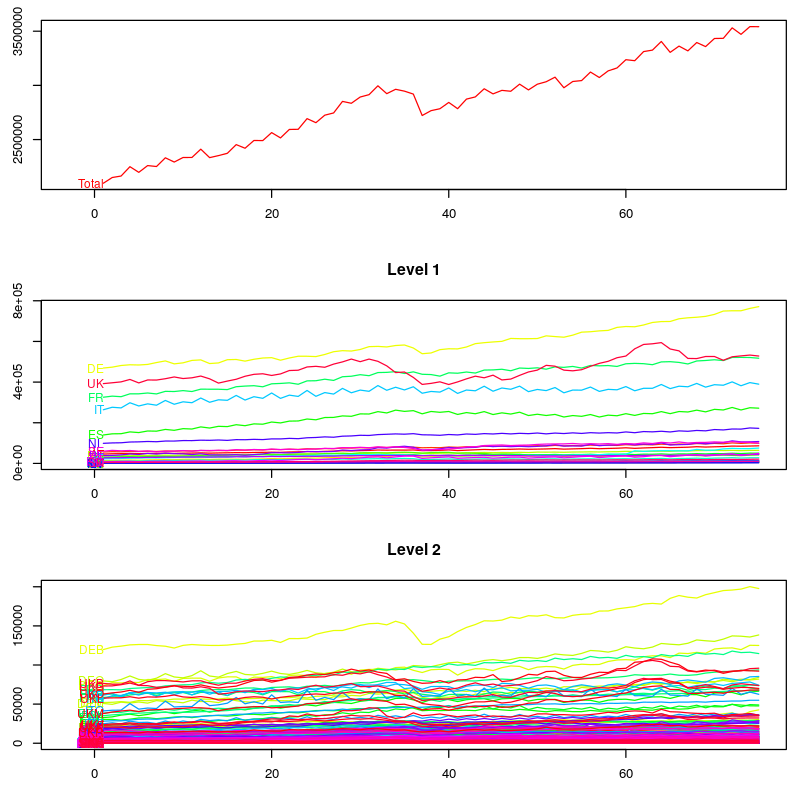
\includegraphics[width=0.7\linewidth]{screenshot001}
%	\caption[Квартальные временные ряды]{Квартальные временные ряды}
%	\label{fig:screenshot001}
%\end{figure}
Разница между совокупным ВВП всех 28 стран, входящих в состав ЕС  и суммой ВДС по всем отраслям для каждого из государств, не превышает  1.5\% от ВВП. 

\subsection{Квартальные сезонно сглаженные данные}

Квартальные сезонно сглаженные данные\footnote{FRED: Economic Data. URL: \url{https://fred.stlouisfed.org/} (дата обращения: 18.02.2019). Код для выгрузки данных с сайта в приложении (A.2).} -- это ряды ВДС  для каждого из 50 штатов Америки с разбивкой на 21 отрасль.  Данные выгружены за период с 2005-Q1 по 2018-Q2. 
В этом наборе 11 рядов имели пропуски. По четырем из этих рядов  данные перестали собираться в 2008 году, поэтому эти ряды были исключены целиком. Остальные пропуски  были заполнены \ \ с \ \ помощью экспоненциально взвешенного скользящего среднего \ \  с \ \  шириной \  \  окна 4\footnote{Алгоритм, используемый в пакете R \texttt{imputeTS}   имеет адаптивный размер окна: в случае длинных промежутков с пропущенными значениями, размер окна постепенно увеличивается до тех пор, пока не появятся как минимум 2 значения не-NA. }. 

Квартальные оценки ВДС в США пересчитываются с учетом сезонных колебаний следующим образом: BEA\footnote{U.S. Bureau of Economic Analysis (BEA). URL: \url{https://www.bea.gov/}  (дата обращения: 25.02.2019) } оценивает соответствующие коэффициенты сезонной корректировки, после чего удаляет из временного ряда среднее влияние изменений, которые обычно происходят примерно в одно и то же время  с одинаковой величиной каждый год. Сезонно несглаженные ряды по этому показателю BEA не публикует.

Показатели по ВДС публикуются в реальном денежном эквиваленте (за базовый год принимается 2012).
Значения реальных показателей ВДС по отраслям не обязательно дают в сумме показатель реального ВДС для каждого штата за интересующий период, поскольку относительные цены, используемые в качестве весов для корректировки показателей по отраслям, отличаются от общего уровня цен используемых для корректировки агрегированного показателя. Эта разница не превышает 0.5\% ВВП.
Для периодов близких к 2012 году, когда значительных отклонений относительных цен от индекса цен по стране не было, показатель ВДС штата совпадает с суммой ВДС по отраслям. 
Разница между ВВП США и суммой ВДС по отраслям для каждого штата не превышает 2\%. 


\subsection{Месячные данные}

Месячные данные -- показатели рождаемости\footnote{ЕМИСС: государственная статистика. Число зарегистрированных родившихся (оперативные данные). URL: \url{https://fedstat.ru/indicator/33555} (дата обращения: 10.04.2019).} и смертности\footnote{ЕМИСС: государственная статистика. Число зарегистрированных умерших по основным классам и отдельным причинам смерти (оперативные данные). URL: \url{https://fedstat.ru/indicator/33559} (дата обращения: 10.04.2019).} по основным причинам  в каждом регионе РФ, дающие в сумме естественный прирост населения помесячно. 
Данные выгружены за период с 2006-01 по 2019-01. 


Если для каждого из регионов все показатели из набора данных <<Число зарегистрированных умерших по основным классам и отдельным причинам смерти>> просуммировать по причинам смерти, значения будут отличаться от показателей  из набора данных <<Число зарегистрированных умерших>>. Такое расхождение объясняется тем, что для перового набора  разрабатываются ряды только по   основным классам и отдельным причинам смерти, имеющим наибольший вес. Также в 2011 году методика разработки показателя была пересмотрена, чтобы соответствовать  международной статистической классификации\footnote{Демографический ежегодник России: методические пояснения. URL: \url{http://www.gks.ru/bgd/regl/B17\_16/Main.htm} (дата обращения: 09.05.2019).}. 

Для анализа необходимы ряды, в сумме дающие агрегированный ряд естественного прироста населения. Для каждого региона имеем следующее разбиение:   



\begin{itemize}
	\item  РО --    число рожденных;
	\item  УБ --  число умерших  из-за болезней (болезней органов дыхания, органов пищеварения, системы кровообращения, инфекционных и паразитарных болезней, новообразований);
\item УУ --   число умерших по причине убийства и самоубийства;
\item УВ --    число умерших по прочим причинам (отравление алкоголем, транспортные травмы всех видов и внешние причины).

\end{itemize}

Три группы причин смертности  были выделены  согласно международной статистической классификации, чтобы избежать большого числа рядов с нулевыми и близкими к нулю значениями.   Разница между показателем смертности по каждому региону и суммой по всем причинам смертности была добавлена к ряду <<УВ>>.


С 2015 года также собираются данные по республике Крым и городу федерального значения Севастополю. Однако данных нужной сезонности по каждому из классов за 2006-2014 годы Держстат Украины\footnote{Держстат Украины -- Статистика населения Украины. URL: \url{http://database.ukrcensus.gov.ua/MULT/Dialog/statfile_c.asp} (дата обращения: 12.05.2019).} не предоставляет, поэтому ряды по этим регионам были исключены из набора данных. 



%- 

\section{Выбор моделей прогнозирования рядов нижнего уровня}

Для того чтобы определить, можно ли с помощью комбинирования прогнозов получить более точные прогнозы агрегированных рядов необходимо выбрать модель для прогнозирования нижних рядов. 
Конечно,   для  каждого  ряда можно подобрать свою модель с параметрами,   оптимизирующими, например, метрику качества прогноза. Недостатками такого метода являются зависимость   от выбора метрики, неинтерпретируемость  результатов     и вычислительная сложность алгоритма, перебирающего все модели для большого числа рядов. Использование одной и той  же модели для всех  рядов иерархии    позволит  увидеть, есть ли зависимость между выбором параметров модели и методом комбинирования рядов или прогнозов.

%Для сравнение качества прогнозов используется кросс-валидация со скользящим окном. 
Эффективность каждого из методов комбинирования будет проверяться на десяти различных моделях: AR с малым числом лагов (с линейным трендом), AR с линейным и с квадратичным трендом, интегрированная AR, ARMA с линейным трендом, ARIMA, 
ETS с фиксированными параметрами,  ARIMA, ETS и TBATS с автоматическим подбором параметров.~\footnote{Автоматический перебор параметров модели осуществляется с помощью функций R  \texttt{auto.arima,ets}  и \texttt{tbats} соответственно. }



Для выбора параметров в моделях применяется кросс-валидация  со скользящим окном с шагом в одно наблюдение. К рядам нижнего уровня будет применяться модель, для которой среднее по всем подвыборкам RMSE, полученное на кросс-валидации для   агрегированного ряда, будет ниже других в классе используемой модели.  





		
Ширина окна для каждого из  наборов данных подбиралась с учетом  длины ряда и горизонта прогнозирования в два года таким образом, чтобы при проведении кросс-валидации с шагом в один год получалось не менее пяти подвыборок. В результате
		\begin{itemize}
			\item для квартальных рядов по ВВП ЕС ширина окна 48, прогноз на 8 шагов вперед;
			\item для  сезонно сглаженных рядов по ВВП США ширина окна 28, прогноз на 8 шагов вперед;
			\item для месячных рядов по естественному приросту РФ ширина окна 84, прогноз на 24 шага вперед.
		\end{itemize}  
		
		
Результат перебора параметров для каждой из основных моделей для всех трех наборов данных представлен в таблице (\ref{tab11}). 		
Для моделей класса ARIMA число лагов  в AR  части   $p$ подбиралось среди значений  меньших или равных  периодичности рядов:  для квартальных -- 4, для месячных -- 12,  число лагов  в  MA  части  $q$  --   меньшее либо равное двум. 	В ETS модели перебирались все возможные  варианты параметров, в TBATS -- тренд мог быть демпфированным, либо нет.   	
Для всех моделей, параметр $\lambda$, отвечающий за преобразование Бокса-Кокса, либо равнялся 1, либо  оценивался в  модели. 
		
		
		Для сравнения качества прогнозов будут использоваться следующие метрики:
		
		\begin{itemize}
			\item  средняя ошибка (mean error):
			\begin{equation}\label{key}
			ME = \frac{1}{h} \sum_{i=1}^h(\hat{y}_{t+i|t}-y_{t+i}) ;
			\end{equation}
			\item  квадратный корень из среднеквадратичной ошибки (root mean square error):
			\begin{equation}\label{key}
			RMSE = \sqrt{  \frac{1}{h} \sum_{i=1}^h(\hat{y}_{t+i|t}-y_{t+i})^2} ;
			\end{equation}
		\end{itemize}
	

		
		\begin{table}[H]
			\caption{Параметры моделей }\label{tab11}
			\small\centering\setlength{\extrarowheight}{0.25em}
			\begin{tabular}%{\linewidth}
				{   >{\centering\footnotesize}p{11em} 
					>{\centering\footnotesize}p{8.5em} 
					>{\centering\footnotesize}p{8.5em} 
					>{\centering\footnotesize\arraybackslash}p{8.5em} }\hline
				
				& Квартальные                                  & Сезонно сглаженные               & Месячные                                      \\\hline
				AR с линейным трендом (с малым числом лагов) & $(p,d,q)=(2,0,0)$,     
				
				$(P,D,Q)_{4}=(1,0,0)$ & $(p,d,q)=(2,0,0)$                & $(p,d,q)=(2,0,0)$,   
				
				$(P,D,Q)_{12}=(1,0,0)$  \\
				AR с линейным 
				
				трендом                        & $(p,d,q)=(3,0,0)$,   
				
				$(P,D,Q)_{4}=(2,0,0)$  & $(p,d,q)=(4,0,0)$                & $(p,d,q)=(11,0,0)$, 
				
				$(P,D,Q)_{12}=(2,0,0)$ \\
				AR с квадратичным 
				
				трендом                    & $(p,d,q)=(3,0,0)$,   
				
				
				$(P,D,Q)_{4}=(2,0,0)$  & $(p,d,q)=(4,0,0)$                & $(p,d,q)=(11,0,0)$,  
				
				$(P,D,Q)_{12}=(2,0,0)$ \\
				Интегрированная AR                            & $(p,d,q)=(3,1,0)$,   
				
				$(P,D,Q)_{4}=(2,1,0)$  & $(p,d,q)=(4,1,0)$                & $(p,d,q)=(4,0,0)$,  
				
				$(P,D,Q)_{12}=(1,1,0)$  \\
				ARMA с линейным 
				
				трендом                      & $(p,d,q)=(3,0,1)$, 
				
				$(P,D,Q)_{4}=(2,0,1)$  & $(p,d,q)=(4,0,1)$                & $(p,d,q)=(4,0,1)$,  
				
				$(P,D,Q)_{12}=(1,0,1)$  \\
				ARIMA                                        & $(p,d,q)=(3,1,1)$,  
				
				$(P,D,Q)_{4}=(2,1,1)$  & $(p,d,q)=(4,1,1)$                & $(p,d,q)=(4,1,1)$, 
				
				$(P,D,Q)_{12}=(1,1,1)$  \\
				ARIMA с автоматическим подбором   параметров           & $\lambda = 1$                                & $\lambda = 1$                    & $\lambda = 1$                                 \\
				ETS с фиксированными параметрами            & $(E,T,S)=(M,M,M)$ 
				
				$\lambda = 1$            & $(E,T,S)=(A,A,A)$ 
				
				$\lambda = 1$ & $(E,T,S)=(A,Ad,A)$ 
				
				$\lambda = 1$             \\
				ETS с автоматическим подбором     параметров           & $\lambda = 1$                                & $\lambda = 1$                    & $\lambda = 1$                                 \\
				TBATS                                        & $\lambda = 1$,  $T=A$                        & $\lambda = 1$,   $T=A$           & $\lambda = 1$,  $T=Ad$                    \\  \hline
				
			\end{tabular}
	
	\
		
		$(p,d,q)$ -- параметры для ARIMA модели, $(P,D,Q)_{m}$ -- параметры для SARIMA модели с периодичностью $m$, $\lambda$ -- параметр преобразования Бокса-Кокса, $T$ - параметр, отвечающий за характер тренда ($A$ - аддитивный, $Ad$ - аддитивный демпфированный, $M$ - мультипликативный)  
		
		\end{table}
		
		
						\begin{itemize}	
			\item  средняя абсолютная ошибка в процентах  (mean absolute percentage error):
			\begin{equation}\label{key}
			MAPE = \frac{1}{h} \sum_{i=1}^h \frac{y_{t+i} - \hat{y}_{t+i|t} }{y_{t+i}} * 100\%.
			\end{equation}
			
		\end{itemize}
		
		
		


%При прогнозировании на два года вперед, получаем 6 подвыборок для США,  6 подвыборок для ЕС,  5 подвыборок для РФ.  

%один год, для сравнения лучших моделей с шагом в одно наблюдение.
%Для выбора параметров в моделях будем использовать кросс-валидацию с шагом в один год, для сравнения лучших моделей с шагом в одно наблюдение.



%\subsection*{Сравнение качества прогнозов}



Основной метрикой сравнения точности прогнозов моделей будет  RMSE. Средняя ошибка (ME) позволит понять, насколько хорошо модель улавливает тренд в рядах.  MAPE в качестве метрики сравнения точности прогнозов является смещенным показателем, поскольку он будет систематически выбирать модель, прогнозы которой занижены, так как на отрицательные ошибки налагаются большие штрафы, чем на положительные. 
Но зато MAPE позволит сравнивать улучшение качества прогнозов для разных наборов данных, хотя  для набора данных по России MAPE не является показательной метрикой, так как в нем имеются нулевые и близкие к нулю значения.


\section{Группировка рядов третьего уровня по регионам, по типу и по кластерам}

Для данного исследования подбирались наборы данных с трехуровневой структурой, обладающие свойством аддитивности. Это позволяет проверить,  можно ли улучшить прогноз агрегированного ряда используя  комбинации прогнозов каждого из рядов третьего уровня или такое  разбиение рядов на слишком большое число компонент излишнее. 
 Если предположить, что разбиение агрегата на компоненты действительно позволяет учесть неоднородность составляющих агрегированного ряда, но оценка большого числа рядов неизбежно приводит к тому, что идиосинкразические    ошибки в сумме растут,     то необходимо найти компромисс между двуми этими эффектами.   
% поскольку приводит к тому, что индивидуальные ошибки прогнозов каждого ряда могут накапливаться, что ведет  к ухудшению прогноза агрегированного ряда.

Очевидно, что можно сгруппировать ряды по территориальному признаку (по странам, штатам или регионам) или по типам (для ВВП группы по отраслям  и для естественного прироста  отдельно ряды по рождаемости, отдельно по основным причинам  смерти). Аддитивность  позволяет получить ряды второго уровня просто просуммировав ряды, входящие в одну группу. 

Альтернативным способом   получение групп является кластеризация.
 Для этого использовался  алгоритм иерархической кластеризации, реализованный в пакете \texttt{dtwclust}. 
Для получения кластеров была выбрана евклидова метрика:
\begin{equation}\label{key}
d(y_{i,t},y_{j,t}) = \sqrt{\sum^T_{t=1} (y_{i,t} - y_{j,t}  )^2 }, 
\end{equation}
где  $y_{i,t},y_{j,t}$ -- ряды нижнего уровня.
Предварительно все ряды нормировались:

\begin{equation}\label{key}
z_{ij,t} = \dfrac{y_{ij,t} - \bar{y}_{ij}}{\sigma(y_{ij})},  
\end{equation}
где $z_{ij,t}$ - нормализованный ряд $y_{ij,t}$.
Оптимальное число кластеров выбиралось так, чтобы максимизировать значение индекса силуэта $SI$ для всей кластерной структуры: 


\begin{equation}\label{key}
SI = \frac{1}{N} \sum^N_{i=1} S_{y_i}=\frac{1}{N} \sum^N_{i=1} \dfrac{b_{pi}-a_{pi}}{\max(a_{pi}, a_{pi})},
\end{equation}
где $N$ -- число кластеров, $S_{y_i}$ -- силуэт каждого элемента, $a_{pi}$ --   среднее расстояние от ряда $y_{pj}$ до других объектов из кластера $y_p$,  $b_{pi}$ --  среднее расстояние от $y_{pj}$ до  объектов из других  кластеров $y_{qj}$,  где  $q\neq p$.
Для всех трех наборов данных оптимальное число кластеров по этой метрике -- 25. Визуализацию рядов попавших в один кластер для квартальных данных представлены на рисунке, для сезонно сглаженных -- на рисунке (\ref{figqq}), для месячных -- на рисунке (\ref{figww}), для всех этих графиков фиолетовые цвета означают значения ряда меньше среднего, зеленые -- выше (\ref{figee}). 



\begin{figure}
	\centering
	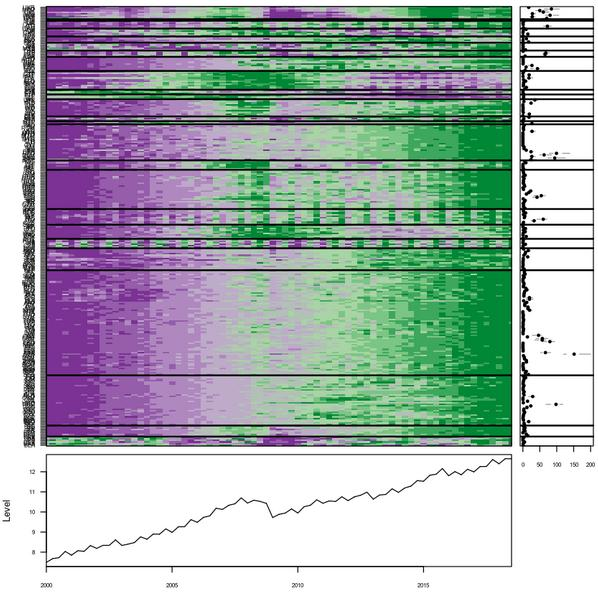
\includegraphics[width=0.6\linewidth]{screenshot014}
	\caption{Временные ряды по ВВП ЕС сгруппированные по евклидовой метрике}
	\label{figqq}
\end{figure}


\begin{figure}
	\centering
	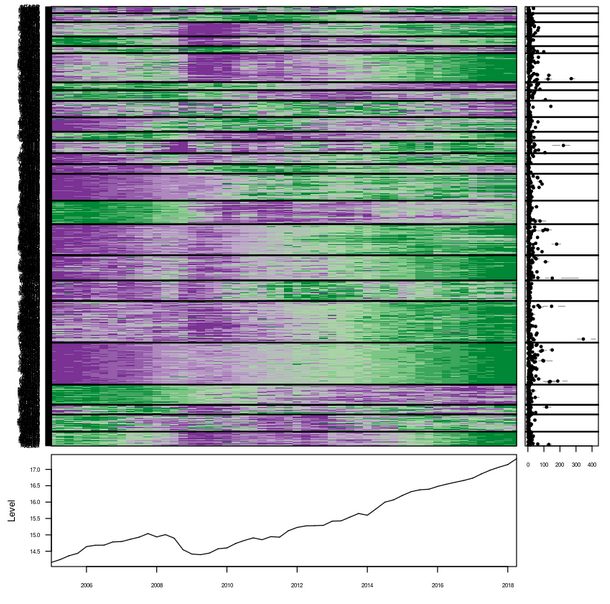
\includegraphics[width=0.6\linewidth]{screenshot015}
	\caption{Временные ряды по ВВП США сгруппированные по евклидовой метрике}
	\label{figww}
\end{figure}

\begin{figure}
	\centering
	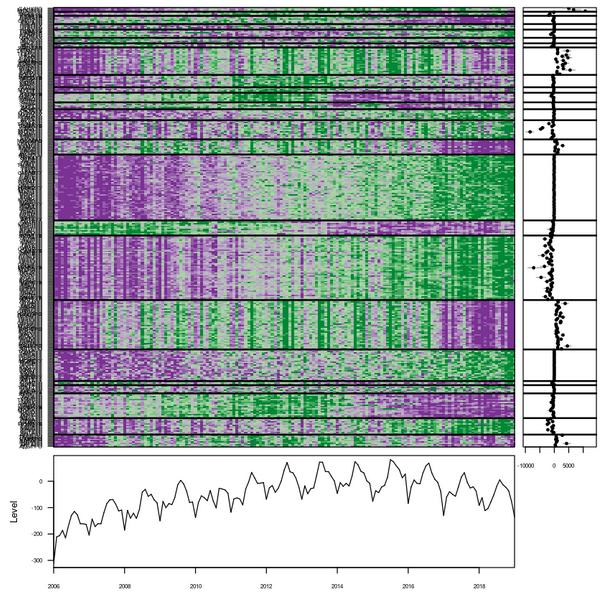
\includegraphics[width=0.6\linewidth]{screenshot016}
	\caption{Временные ряды по естественному приросту РФ сгруппированные по евклидовой метрике}
	\label{figee}
\end{figure}


При использовании процедуры кросс-валидации необходимо было на каждой итерации получать свою группировку на  кластеры, но с целью проверки для экономии времени проведем кластеризацию на рядах полной длины.



%https://cran.r-project.org/web/packages/dtwclust/vignettes/dtwclust.pdf

%https://cran.r-project.org/web/packages/dtwclust/dtwclust.pdf



\section{Сравнение иерархических моделей}

Для сравнения моделей используется следующая процедура\footnote{Все коды необходимые для проведения описанной процедуры выложены сайте GitHub. URL: \url{https://github.com/xenakas/disaggregated_ts}  }: 

\begin{itemize}
	\item разбиение рядов на подвыборки для выполнения кросс-валидации со скользящим окном с шагом в один год: для квартальных данных число подвыборок равно 6, для сезонно сглаженных -- 6, для месячных -- 5;
	%При прогнозировании на два года вперед, получаем 6 подвыборок для США,  6 подвыборок для ЕС,  5 подвыборок для РФ.  	
	\item модели описанные в таблице (\ref{tab11}) используются для получения прогноза на 2 года вперед для каждого ряда, каждого уровня  (отдельно с помощью пакета \texttt{hts} оценивается   трехуровневая модель,  отдельно три двухуровневые: сгруппированные по регионам, по классам или по кластерам);
	\item на каждой итерации кросс-валидации считается RMSFE для агрегированного ряда, RMSFE для невзвешенной суммы всех прогнозов нижнего ряда и RMSFE для скорректированной по OLS суммы всех прогнозов;
	\item для каждого набора данных RMSFE усредняется по  всем подвыборкам и считается процентное изменение  RMSFE для невзвешенной суммы и скорректированной по OLS суммы всех прогнозов по сравнению с RMSFE для агрегированного ряда;
	\item полученные значения для трехуровневой и двухуровневых моделей сортируются по  RMSFE   для агрегированного ряда.
\end{itemize}


По результатам полученным с помощью   описанной процедуры формируются таблицы на которых можно  увидеть, как изменился прогноз агрегированного ряда при использовании моделей, учитывающих многоуровневую  структуру данных (Приложение (\ref{app-b})). Для наглядности при относительном уменьшении RMSFE ячейка таблицы окрашивается в зеленый, при относительном увеличении -- в красный. Цвета также отличаются по интенсивности, чем ярче, тем больше отклонение от RMSFE полученного по прогнозам для агрегированного ряда.

При анализе  полученных показателей  и визуального  представления  наборов данных (Приложение (\ref{app-a}))  были получены три основных  вывода:
эффективность иерархических  моделей  сильно варьируется в зависимости от структуры рядов-компонент;
комбинирование прогнозов с помощью OLS-корректировки  позволяет устранить сильное отклонение невзвешенной суммы прогнозов от прогноза агрегированного, появившееся из-за случайного накопления идиосинкразических ошибок;
предварительная группировка рядов нижнего уровня перед прогнозированием практически во всех случаях приносит положительный результат, по сравнению с прогнозами полученными по трехуровневой модели. 





%\subsection*{Вывод 1:}

Опишем подробнее полученные результаты и причины, по которым были сделаны соответствующие выводы.
Для невзвешенных прогнозов результаты неоднозначны: для квартальных данных в большинстве случаев при использовании иерархических моделей наблюдается ухудшение  по сравнению прогнозом агрегированного ряда (\ref{fig111}), для сезонно сглаженных рядов для большинства моделей наблюдается улучшение прогнозов (\ref{fig222}), а для месячных на некторых моделях наблюдается улучшение для всех вариантов структуры (трех- и двухуровневой),   на некоторых -- ухудшение (\ref{fig333}).
 
 
\begin{figure}
	\centering
	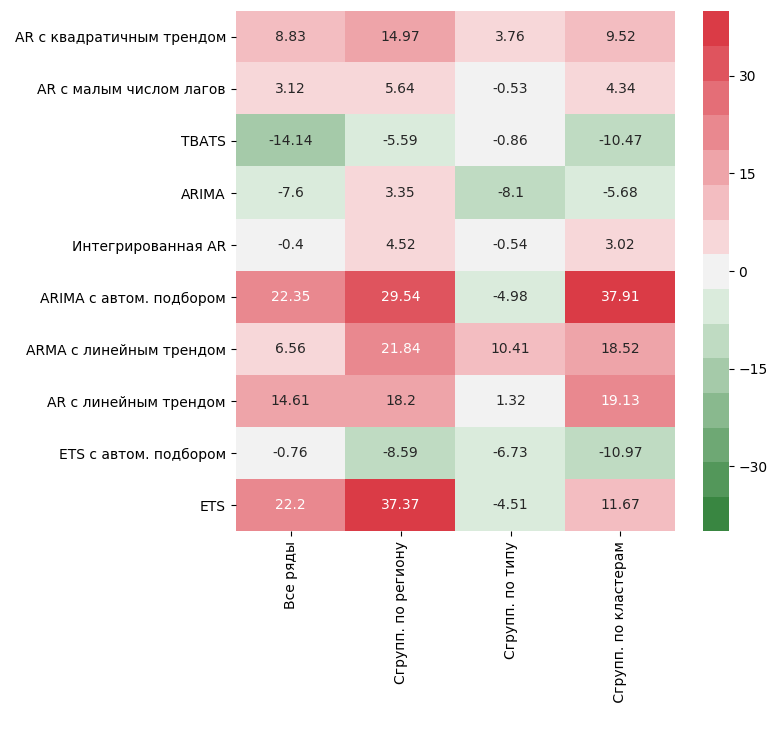
\includegraphics[width=0.7\linewidth]{screenshot020}
	\caption{Процентное изменение RMSE (невзвешенные прогнозы, квартальные ряды).
	}
	\label{fig111}
\end{figure}
 
\begin{figure}
	\centering
	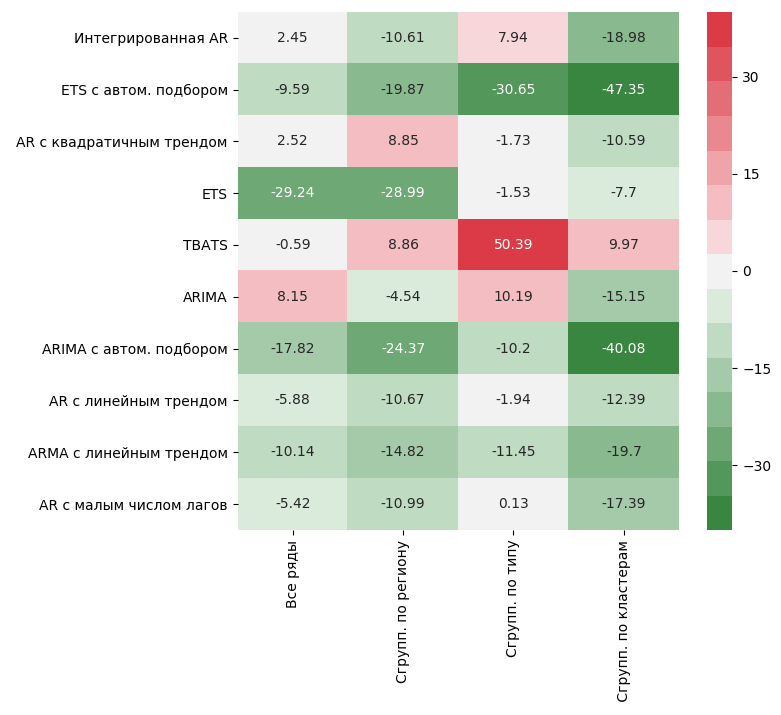
\includegraphics[width=0.7\linewidth]{screenshot021}
	\caption{Процентное изменение RMSE (невзвешенные прогнозы, сезонно сглаженные  ряды).
	}
	\label{fig222}
\end{figure}

 
\begin{figure}
	\centering
	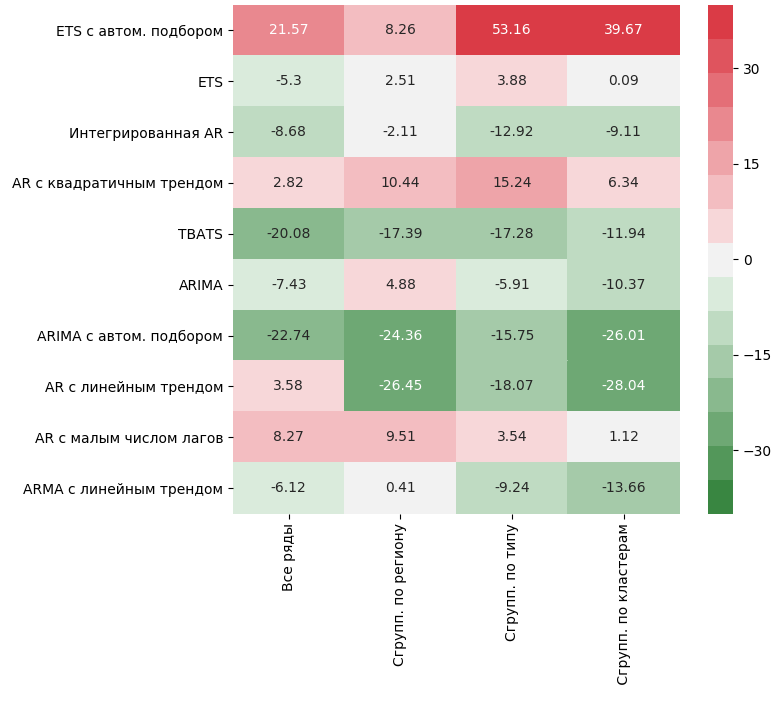
\includegraphics[width=0.7\linewidth]{screenshot022}
	\caption{Процентное изменение RMSE (невзвешенные прогнозы, месячные ряды).
	}
	\label{fig333}
\end{figure}

 
 
	Возможно это объяснется следующими фактами. Для квартальных данных все ряды имеют примерно одинаковую структуру и  ошибки прогнозов не уравновешивают друг друга, а накапливаются.  Для сезонно сглаженных рядов для всех итераций кросс-валидации  метрика ME значительно больше нуля,  то есть на всех итерациях  модель в среднем занижает прогнозы. При прогнозировании отдельных компонент  с этим  можно бороться, поскольку только малая часть прогнозов рядов приводит к тому, что тренд недооценивается, и эти прогнозы выравниваются большим числом прогнозов улавливающих положительный тренд.     Для месячных данных причина неоднозначных результатов заключается в   том, что примерно четверть рядов имеет $\cap$-образный тренд (ряды по рождаемости), половина положительный линейный тренд, четверть отрицательный линейный тренд (что видно на рисунке (\ref{fig224}),   где ряды группируются по типу).  Соответственно для некоторых моделей хорошие  прогнозы  имела большая по размеру группа, а для некоторых меньшая.
	
	\begin{figure}
		\centering
		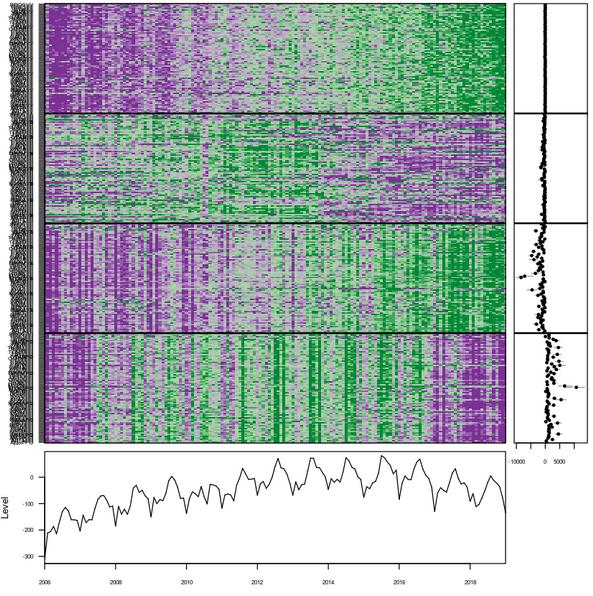
\includegraphics[width=0.7\linewidth]{screenshot013}
		\caption{Месячные ряды, сгруппированные по типу.
		}
		\label{fig224}
	\end{figure}
	
	
	
%\subsection*{Вывод 2:}

Прогнозы полученные с помощью OLS  корректировки  для квартальных и сезонно сглаженных рядов в большинстве случаев  не отличаются от прогнозов полученных при прогнозировании агрегированного ряда. Доля  прогнозов нижних рядов значительно отличающихся  от  прогнозов верхних рядов оказалась небольшой, поэтому оценки для агрегата скорректировались незначительно.   

Для невзвешенных  прогнозов наблюдалось  резкое  ухудшение для квартальных и резкое улучшение для сезонно сглаженных рядов, но при корректировке эти резкие изменения сгладились (рисунки (\ref{fig112})), (\ref{fig223}))). Учитывая это можно сказать, что при небольшом числе наблюдений, недостаточном для проведения кросс-валидации, стоит    использовать OLS корректировку   прогнозов. Это позволит избежать резких отклонений от настоящих значений ряда, произошедших из-за случайного накопления ошибок. Накопление ошибок может привести, как  к положительному эффекту, так и к отрицательному результату. 
%Применительно к полученным резульатам можно, что можно наблюдать на прогнозах по квартальным данным, где использование моделей с иерархической структурой в  .

 
\begin{figure}
	\centering
	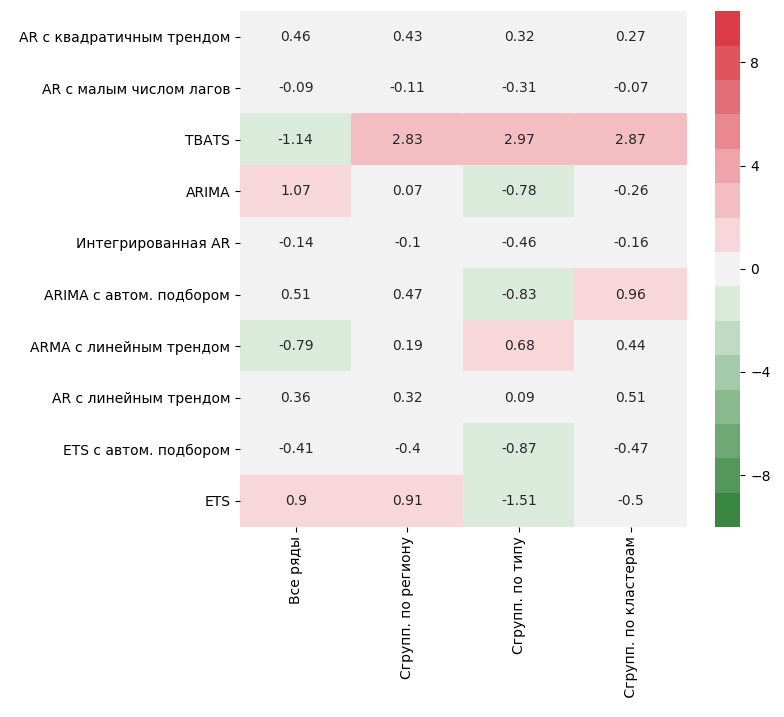
\includegraphics[width=0.7\linewidth]{screenshot017}
	\caption{Процентное изменение RMSE (OLS - скорректированные прогнозы, квартальные ряды).
	}
	\label{fig112}
\end{figure}

\begin{figure}
	\centering
	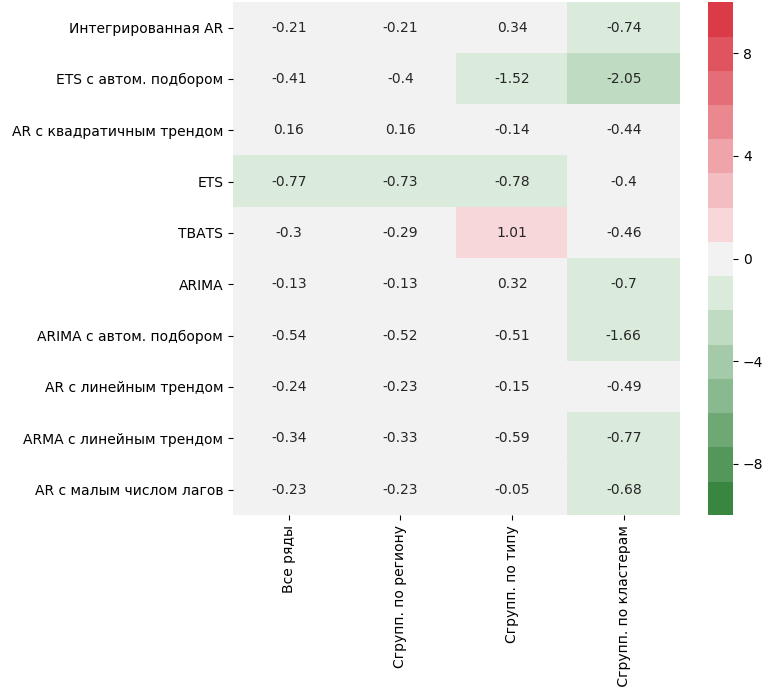
\includegraphics[width=0.7\linewidth]{screenshot018}
	\caption{Процентное изменение RMSE (OLS - скорректированные прогнозы, сезонно сглаженные  ряды).
	}
	\label{fig223}
\end{figure}


\begin{figure}
	\centering
	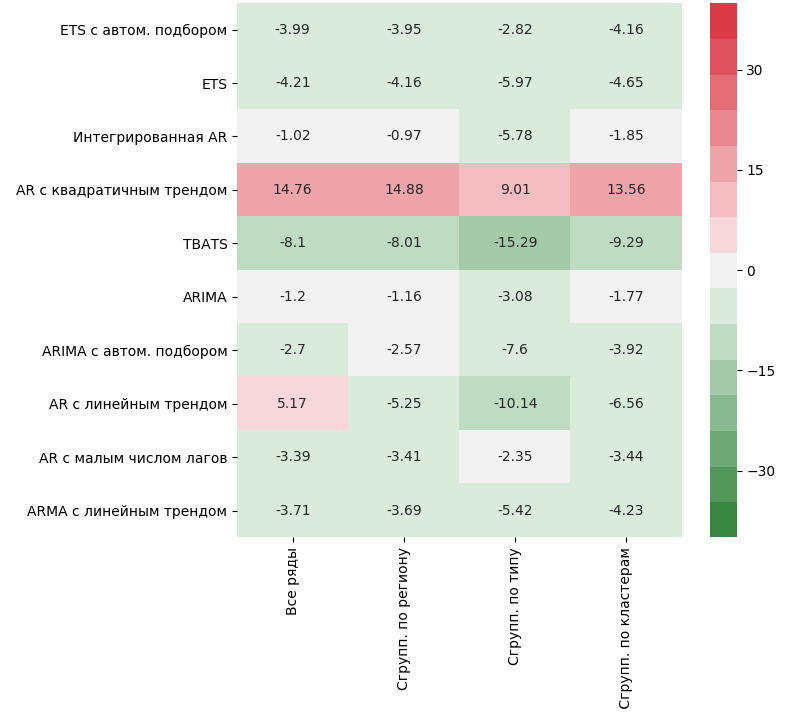
\includegraphics[width=0.7\linewidth]{screenshot019}
	\caption{Процентное изменение RMSE (OLS - скорректированные прогнозы, месячные ряды).
	}
	\label{fig334}
\end{figure}




Для месячных данных при OLS корректировке в отличие от     невзвешенной суммы прогнозов  практически для любой модели наблюдается уменьшение RMSE по сравнению с  RMSE для  агрегированного ряда. Исключение составляет только модель с квадратичным трендом. Причина этому заключается в том, что только четверть рядов имеют $\cap$-образную форму, такую же, как у  агрегированного  ряда.  Поэтому корректировка прогнозов агрегированного ряда на априори худшие  прогнозы по рядам  имеющим  значительно  отличающийся тренд  приводит к тому, что прогнозы сильно корректируются в сторону ухудшения. 
%По той же причине для AR модели с большим числом лагов с линейным трендом для модели с трехуровневой структурой наблюдается ухудшение, поскольку треть рядов прогнозируется по подходящей модели, а четверть по распределению  совпадает   с некачественным агрегированным прогнозом.  

%\subsection*{Вывод 3:}

Если сравнивать эффективность использования различных видов  группировки можно сказать, что  в среднем ее использование  перед получением прогнозов отдельных рядов приносит положительный результат. Причем для квартальных данных лучше всего работает группировка по отраслям (как со взвешиванием, так и без), для сезонно сглаженных для обоих способов  заметное улучшение наблюдается при группировке по кластерам,  для месячных данных для невзвешенных прогнозов более эффективна группировка по кластерам, а для взвешенных -- группировка по типам.

В модели с  комбинированием прогнозов согласно уравнению линейной регрессии (\ref{abc}),
корректировка происходила с учетом 
трехуровневой структуры, где ряды второго уровня собирались  именно по территориальному признаку. При анализе сравнительных таблиц по моделям было выявлено, что для всех наборов данных группировка по различным признакам приводит к неодинаковым результатам. По этой причине  имело бы смысл проводить OLS корректировку прогнозов по суммирующей матрице, учитывающей, что на втором уровне иерархической структуре будут ряды, сгруппированные по наиболее подходящему  для каждого набора данных признаку. 



Во всех случаях группировка по территориальному признаку оказывалась чуть хуже других типов группировок и по отношению к трехуровневой модели без группировки улучшение происходило не во всех случаях.  
При группировке по этому признаку ряды не содержат  в себе информацию о структуре, составляющих их компонент. Если группы по типам ведут себя похожим образом, то деления на регионы  достаточно, чтобы улучшить прогнозы агрегированного ряда.      Но в некоторых случаях, например, для месячных данных,  ряды четко делятся на  небольшое число групп примерно равного размера, потеря этой информации ведет к ухудшению прогнозов.  Также деление рядов по географическому признаку может  усилить эффект накапливания индивидуальных ошибок из-за неучтенной пространственной зависимости. 

При группировке по типу число рядов второго уровне получается меньше, чем при группировке по территориальному признаку или по кластерам.  Эти  ряды не только статистически   похожи друг на друга, но и имеют схожий экономический смысл. Логично предположить, что  реакция таких рядов  на внешние непрогнозируемые шоки с большей вероятностью будет похожей. 

Группировка по кластерам в общем  приносит положительные результаты, однако нельзя забывать, что за определенный отрезок  времени ряды могли случайно попасть в один кластер, поскольку согласно выбранной метрике кластеризации учитывалась только близость нормированных рядов без учета каких-либо экономических факторов. По этой причине то, что  в некоторых случаях  прогнозы полученные после группировки по кластерам оказывалась хуже других, можно объяснить  тем, что  алгоритм  уловил зависимости, которых на самом деле нет.  



%\begin{table}[ht]
%	\centering
%	\begin{tabular}{rrrrr}
%		\hline
%		& ME & RMSE & MAPE & MASE \\ 
%		\hline
%		RW with drift  & 0.02 & 34.78 & 0.82 & 0.29 \\ 
%		Auto ARIMA & 70.50 & 71.55 & 2.03 & 0.73 \\ 
%		ARIMA & 72.67 & 73.73 & 2.09 & 0.75 \\ 
%		RW & 77.53 & 100.92 & 2.52 & 0.91 \\ 
%		ETS & 100.50 & 108.39 & 2.87 & 1.04 \\ 
%		Theta & 103.38 & 109.50 & 2.96 & 1.07 \\ 
%		SNaive & 134.86 & 146.04 & 3.86 & 1.40 \\ 
%		\hline
%	\end{tabular}
%\end{table}
%
%\begin{tabular}{rrrrr}
%	\hline
%	& ME & RMSE & MAPE & MASE \\ 
%	\hline
%	RW with drift  & 0.02 & 34.78 & 0.82 & 0.29 \\ 
%	Auto ARIMA & 70.50 & 71.55 & 2.03 & 0.73 \\ 
%	ARIMA & 72.67 & 73.73 & 2.09 & 0.75 \\ 
%	RW & 77.53 & 100.92 & 2.52 & 0.91 \\ 
%	ETS & 100.50 & 108.39 & 2.87 & 1.04 \\ 
%	Theta & 103.38 & 109.50 & 2.96 & 1.07 \\ 
%	SNaive & 134.86 & 146.04 & 3.86 & 1.40 \\ 
%	\hline
%\end{tabular}
%



\chapter*{Заключение}
\addcontentsline{toc}{chapter}{Заключение}



В этом исследовании продемонстрированы различные подходы к прогнозированию временных рядов с многоуровневой иерархической структурой, позволяющие учитывать взаимозависимости как между самими рядами, так и между  прогнозами. 
%Эффективность этих методов проверялась на трех различных наборов данных, длина рядов в которых позволяла проводить кросс-валидацию.
%Проведенное исследование показало, что используя  иерархические моделей можно  провести анализ и улучшить прогнозы наборов данных со  структурой.



В результате проведенного анализа были получены три основных вывода: 

\begin{itemize}
	\item эффективность   прогнозирования  агрегированных рядов с помощью моделей, учитывающих многоуровневую структуру данных,  сильно варьируется в зависимости от структуры наборов данных и характеристик рядов-компонент   по отдельности;
	\item комбинирование прогнозов с помощью OLS-корректировки  имеет смысл при небольшом числе наблюдений, недостаточном для проведения кросс-валидации, поскольку позволяет устранить сильное отклонение невзвешенной суммы прогнозов от прогноза агрегированного ряда по причине случайного накопления идиосинкразических ошибок;
	\item     предварительная группировка рядов нижнего уровня перед прогнозированием практически во всех случаях дает положительный результат, по сравнению с прогнозами полученными по трехуровневой модели. 
\end{itemize}


% Помимо этого существует и межвременная агрегация временных рядов, часто применяющаяся при прогнозировании.  



%Взвешивание прогнозов повышает точность прогнозов, по сравнению с невзвешенной суммой прогнозов рядов третьего уровня

%Прогнозирование рядов второго уровня дает сопоставимые прогнозы с прогнозом агрегированного ряда, если спецификация модели ряда первого уровня совпадает со спецификацией его компонент. 






% теоретическую и практическую значимость работы (если работа претендует на значи-мые результаты в этих аспектах)

%Практическая значимость работы заключается в том, что при анализе результатов применения изучаемых методов на трех наборах данных (с разной сезонностью, числом наблюдений и рядов на каждом уровне)   с использованием перекрестной проверки (кросс-валидации) можно протестировать методы на независимых данных, а следовательно получить более устойчивые  выводы. 





\newpage

\nocite{*}  %Чтобы в список литературы напечаталичь все источники из bib-файла

% Если нам хочется, чтобы в списке литературы были не полуторные интервалы можно воспользоваться следующим приёмом: 
\begingroup
\setstretch{1}
\addcontentsline{toc}{chapter}{Список литературы}

\printbibliography[title = Список литературы]

\endgroup







%%%%%%%%%%%%%%%%%%%% Приложения %%%%%%%%%%%%%%%%%%%%

\appendix
\renewcommand{\thechapter}{\Asbuk{chapter}}

%%%%%%%%%% titlesec для приложений
\titleformat{\chapter}
 {\normalfont\bfseries\large}{\chaptertitlename~\thechapter}{0.25em}{\normalfont}


\titlecontents{chapter}
              [0 em] % 
              {\normalsize}
              {\makebox[7em][l]{Приложение \thecontentslabel}}
              {Приложение }
              {\titlerule*[10pt]{.}\contentspage}


\chapter[Коды для выгрузки данных]{Коды для выгрузки данных}\label{app-b}

\section*{A.1 Код для выгрузки данных с Eurostat }

\begin{verbatim}
library(eurostat)
library(lubridate)

a10 <- get_eurostat(id="namq_10_a10", time_format="date")
a10 <- subset(a10, a10$s_adj=='NSA') # Unadjusted data 
a10 <- subset(a10, a10$na_item=='B1G') #Value added, gross
a10 <- subset(a10, a10$unit=='CP_MEUR') #Current prices, million euro

a10$unit <- NULL
a10$s_adj <- NULL
a10$na_item <- NULL

gdp <- get_eurostat(id="namq_10_gdp", time_format="date")
gdp <- subset(gdp, gdp$s_adj=='NSA') # Unadjusted data 
gdp <- subset(gdp, gdp$na_item=='B1G') #Value added, gross
gdp <- subset(gdp, gdp$unit=='CP_MEUR') #Current prices, million euro

gdp$unit <- NULL
gdp$s_adj <- NULL
gdp$na_item <- NULL

write.csv(a10, file = "a10_unstacked.csv")
write.csv(gdp, file = "eu_gdp_unstacked.csv")
\end{verbatim}
\newpage





\section*{A.2 Код для выгрузки данных с FRED }

\begin{verbatim}
library(fredr)
library(purrr)
fredr_set_key("bd4355a0bcb45a05a7280e4d99a4d146")
readRDS("states.rds")
readRDS("industries.rds")

dict = c()
for (state in states){
     data = fredr_series_search_text(search_text = 
     paste("Real Gross Domestic Product by Industry", state ), 
     filter_variable = "frequency", filter_value = "Quarterly") 
     data = subset(data, units == "Millions of Chained 2012 Dollars")
     dict = rbind(dict, data.frame(data$id, data$title)  )
}

id_list = as.character(dict$data.id)
gdp_us = c()
for (id in id_list){
     gdp_us = rbind(gdp_us, fredr(series_id = id )  )
	}

data = fredr_series_search_text(search_text = paste("Real Gross 
Domestic Product") , filter_variable = "frequency", 
filter_value = "Quarterly") 
data = subset(data, units == "Millions of Chained 2012 Dollars")
data = fredr_series_search_text(search_text = paste("Real Gross Domestic 
Product") , filter_variable = "frequency", filter_value = "Quarterly") 
data = subset(data, units == "Billions of Chained 2012 Dollars")
data = subset(data, seasonal_adjustment == "Seasonally Adjusted Annual Rate")

gdp_us = fredr(series_id = 'GDPC1' ) 
gdp_us$series_id  <- NULL

write.csv(data, file = "naus_labelled.csv")
write.csv(gdp_us, file = "new_gdp_total.csv")
\end{verbatim}



\newpage



\chapter[Визуализация временных рядов с трехуровневой структурой]{Визуализация временных рядов с трехуровневой структурой}\label{app-a}
\begin{figure}[H]
	\caption{Временные ряды полученные путем агрегирования рядов третьего уровня }
	\label{otkl_1}

	\centering\footnotesize{Квартальные данные -- ВВП ЕС }
		
	\begin{minipage}[H]{0.4\linewidth}
		\centering{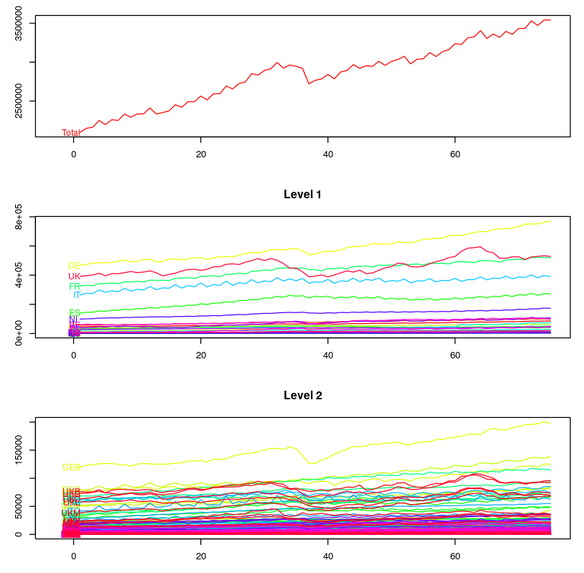
\includegraphics[width=1\linewidth]{screenshot002}}
	\end{minipage}
	\begin{minipage}[H]{0.4\linewidth}
		\centering{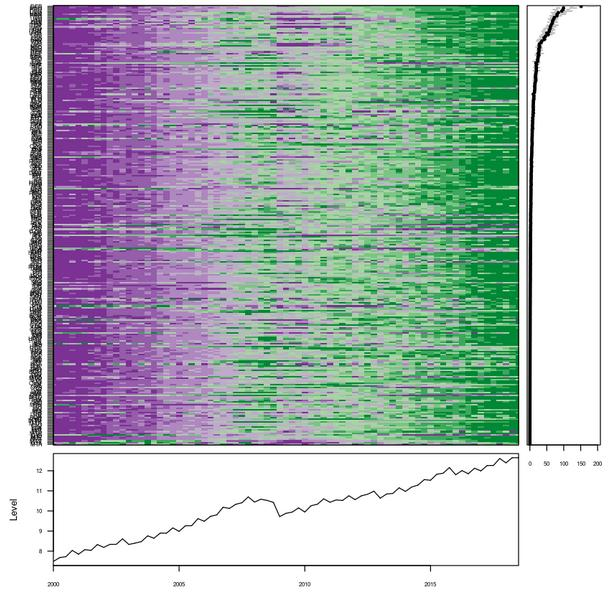
\includegraphics[width=1\linewidth]{screenshot005}}
	\end{minipage}


	\centering\footnotesize{Сезонно сглаженные данные -- ВВП США}
	
	\begin{minipage}[H]{0.4\linewidth}
		\centering{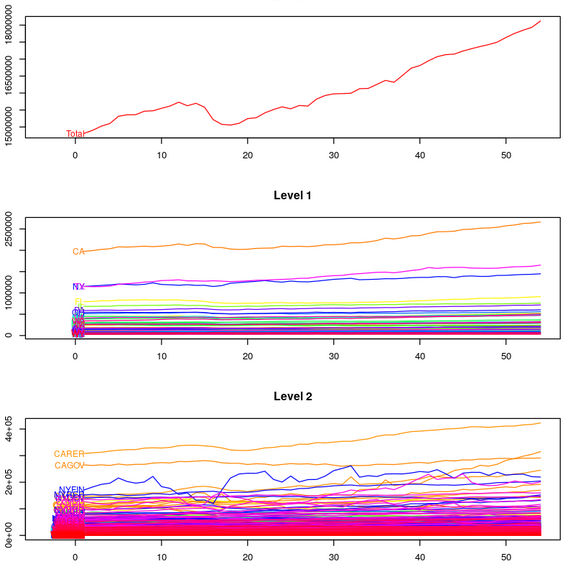
\includegraphics[width=1\linewidth]{screenshot003}}
	\end{minipage}
\begin{minipage}[H]{0.4\linewidth}
	\centering{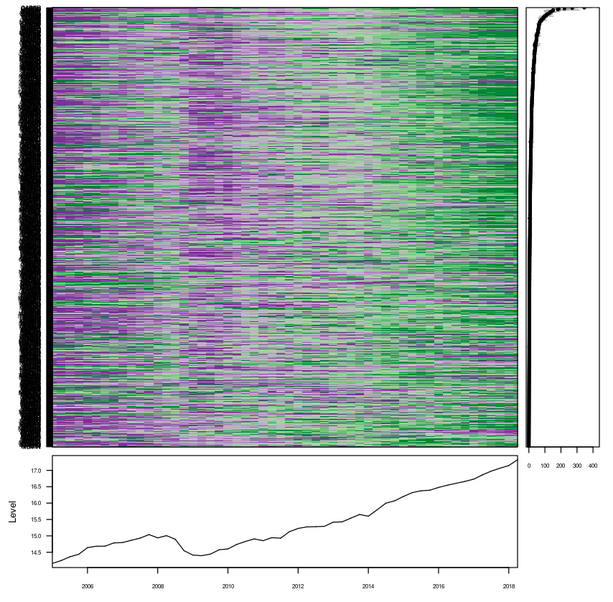
\includegraphics[width=1\linewidth]{screenshot006}}
\end{minipage}


	\centering\footnotesize{Месячные данные -- естественный прирост РФ  }
	
	\begin{minipage}[H]{0.4\linewidth}
		\centering{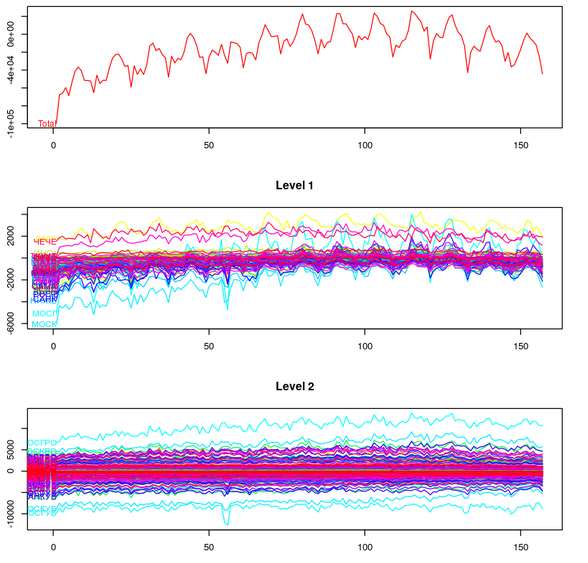
\includegraphics[width=1\linewidth]{screenshot004}}
	\end{minipage}
%	\hfill
\begin{minipage}[H]{0.4\linewidth}
	\centering{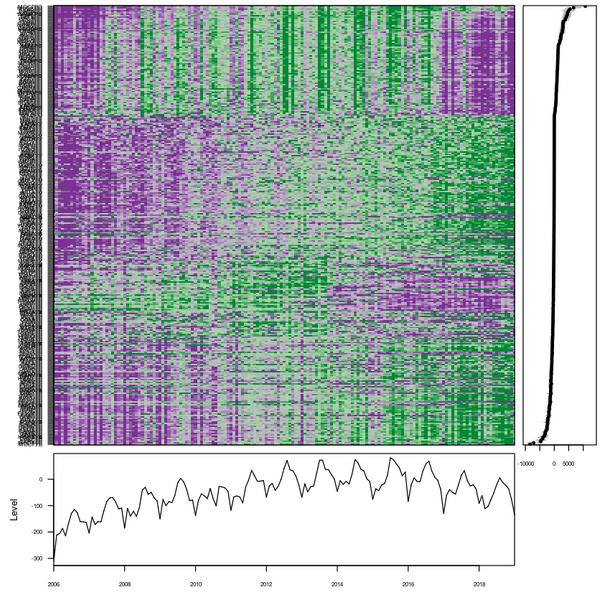
\includegraphics[width=1\linewidth]{screenshot007}}
\end{minipage}
\end{figure}
\newpage



\begin{figure}[H]
	\caption{Временные ряды сгруппированные по территориальному признаку и  по типу }
	\label{qwe}
	
	\centering\footnotesize{Квартальные данные -- ВВП ЕС  }
	
	\begin{minipage}[H]{0.4\linewidth}
		\centering{\footnotesize{по 28 странам  }
			\\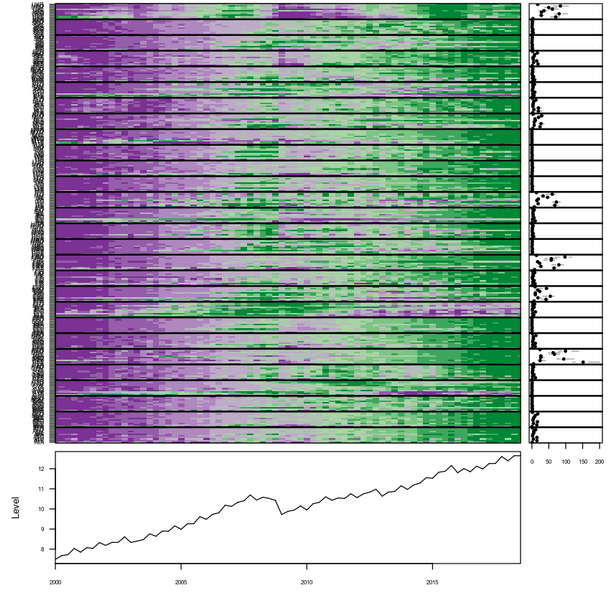
\includegraphics[width=1\linewidth]{screenshot008}}
	\end{minipage}
	\begin{minipage}[H]{0.4\linewidth}
		\centering{\footnotesize{по 10 отраслям  }
			\\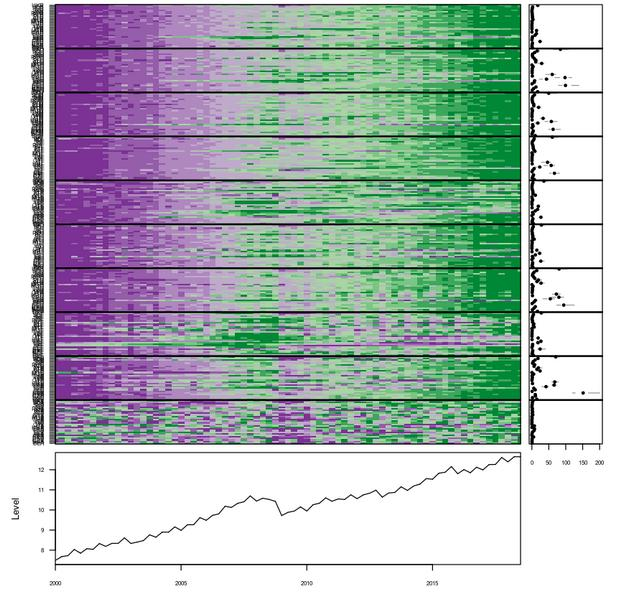
\includegraphics[width=1\linewidth]{screenshot009}}
	\end{minipage}
	
	
	\centering\footnotesize{Сезонно сглаженные данные -- ВВП США}
	
	\begin{minipage}[H]{0.4\linewidth}
		\centering{\footnotesize{по 50 штатам  }
			\\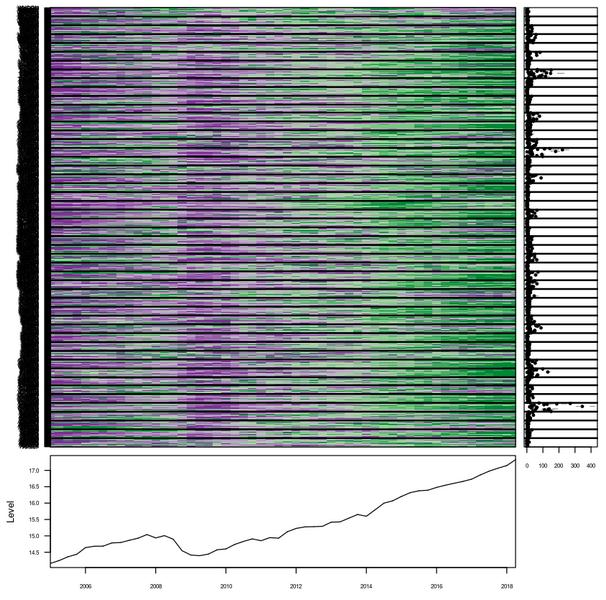
\includegraphics[width=1\linewidth]{screenshot010}}
	\end{minipage}
	\begin{minipage}[H]{0.4\linewidth}
		\centering{\footnotesize{по 21 отрасли   }
			\\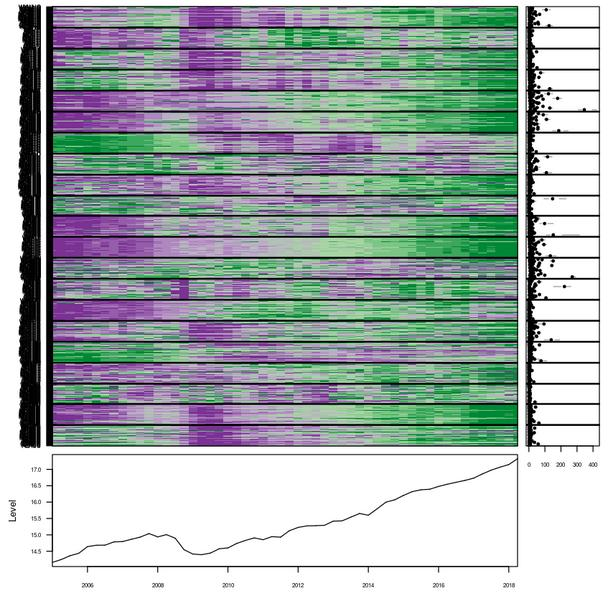
\includegraphics[width=1\linewidth]{screenshot011}}
	\end{minipage}
	
	
	\centering\footnotesize{Месячные данные -- естественный прирост РФ  }
	
	\begin{minipage}[H]{0.4\linewidth}
		\centering{\footnotesize{по 80 регионам }
			\\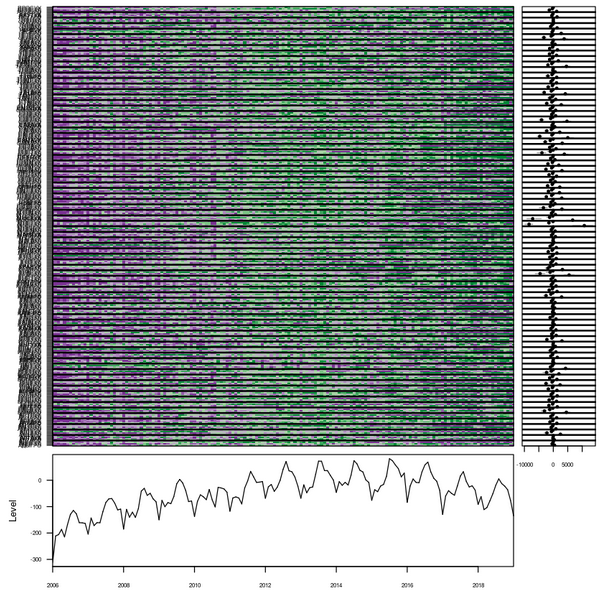
\includegraphics[width=1\linewidth]{screenshot012}}
	\end{minipage}
	%	\hfill
	\begin{minipage}[H]{0.4\linewidth}
		\centering{\footnotesize{по 4 классам   }
			\\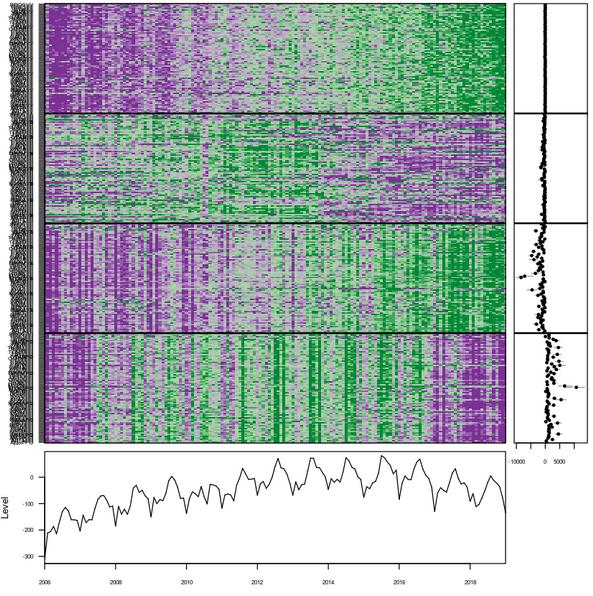
\includegraphics[width=1\linewidth]{screenshot013}}
	\end{minipage}
\end{figure}
\newpage



\chapter[Сравнение иерархических моделей]{Сравнение иерархических моделей}\label{app-b}


\begin{figure}[H]
	\caption{Таблицы, указывающие на процентное изменение RMSE иерархических моделей по сравнению с RMSE моделей прогнозирования  агрегированного ряда   }
	\label{otkl_1}
	
	\centering\footnotesize{Квартальные данные -- ВВП ЕС  }
	
	\begin{minipage}[H]{0.4\linewidth}
		\centering{\footnotesize{невзвешенные прогнозы}
			\\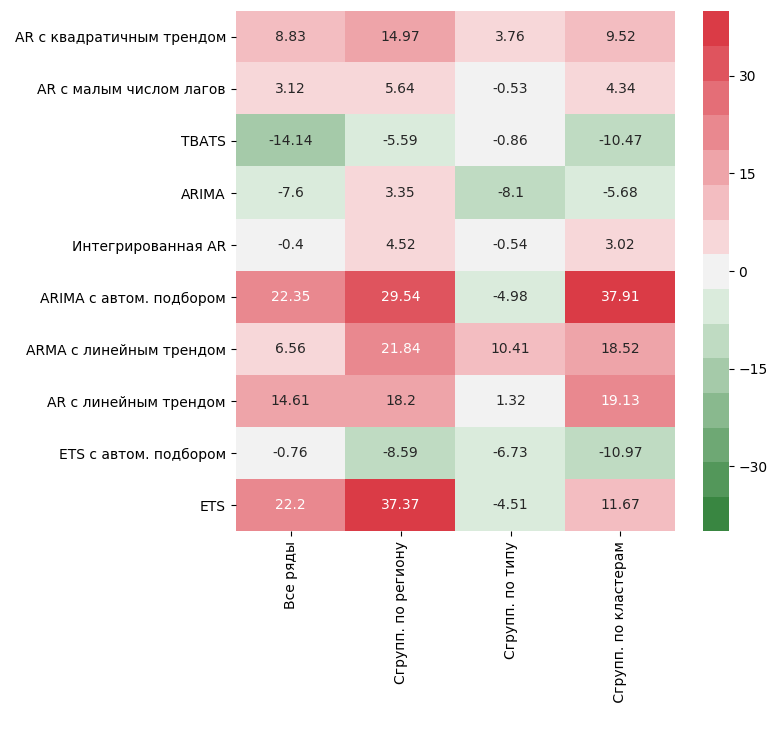
\includegraphics[width=1\linewidth]{screenshot020}}
	\end{minipage}
		\hfill
	\begin{minipage}[H]{0.4\linewidth}
		\centering{\footnotesize{ OLS взвешенные прогнозы }
			\\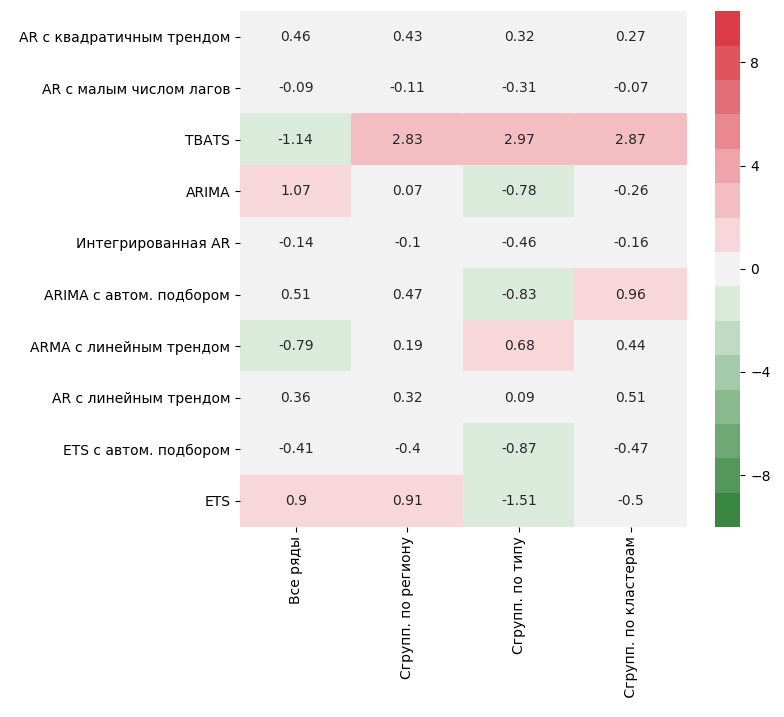
\includegraphics[width=1\linewidth]{screenshot017}}
	\end{minipage}
	
	
	\centering\footnotesize{Сезонно сглаженные данные -- ВВП США}
	
	\begin{minipage}[H]{0.4\linewidth}
		\centering{\footnotesize{невзвешенные прогнозы  }
			\\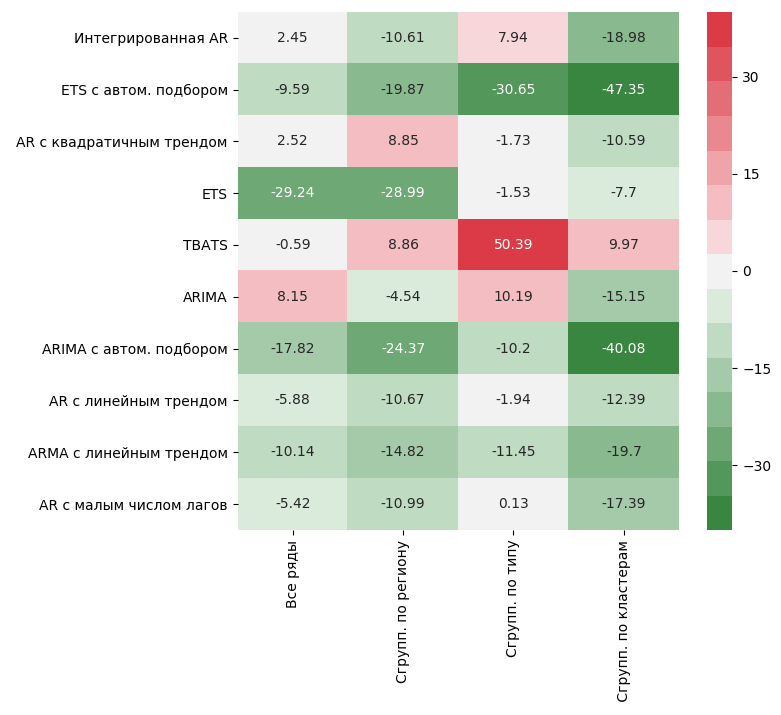
\includegraphics[width=1\linewidth]{screenshot021}}
	\end{minipage}
		\hfill
	\begin{minipage}[H]{0.4\linewidth}
		\centering{\footnotesize{OLS взвешенные прогнозы  }
			\\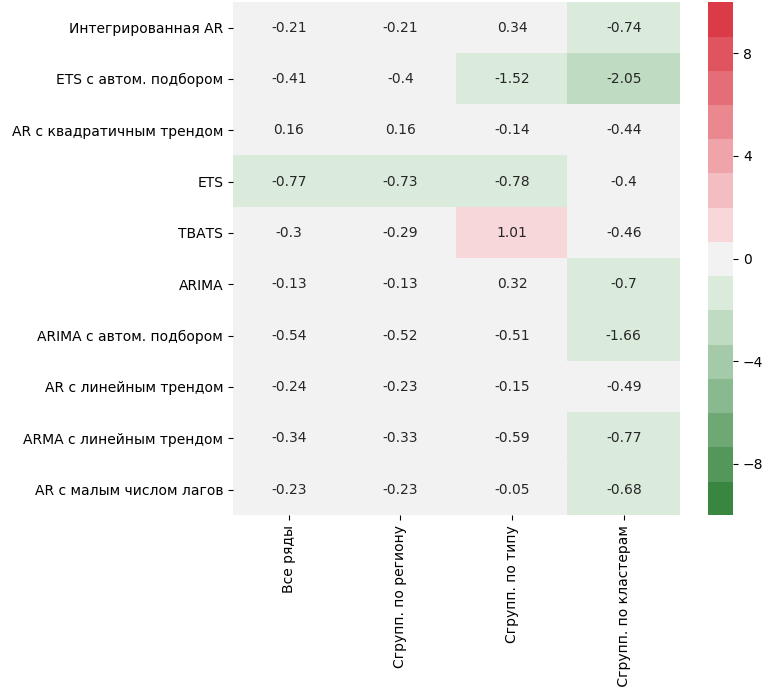
\includegraphics[width=1\linewidth]{screenshot018}}
	\end{minipage}
	
	
	\centering\footnotesize{Месячные данные -- естественный прирост РФ  }
	
	\begin{minipage}[H]{0.4\linewidth}
		\centering{\footnotesize{невзвешенные прогнозы }
			\\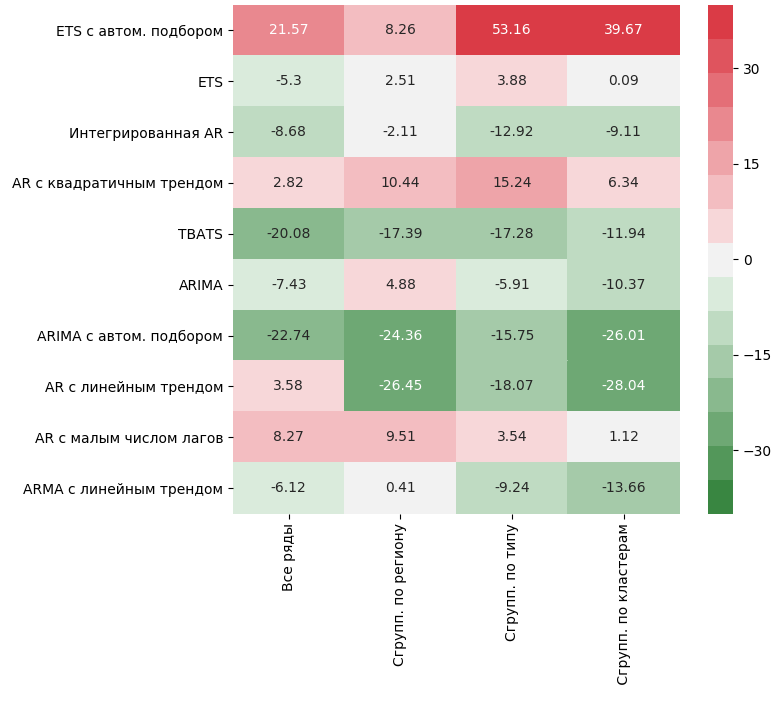
\includegraphics[width=1\linewidth]{screenshot022}}
	\end{minipage}
		\hfill
	\begin{minipage}[H]{0.4\linewidth}
		\centering{\footnotesize{OLS взвешенные прогнозы }
			\\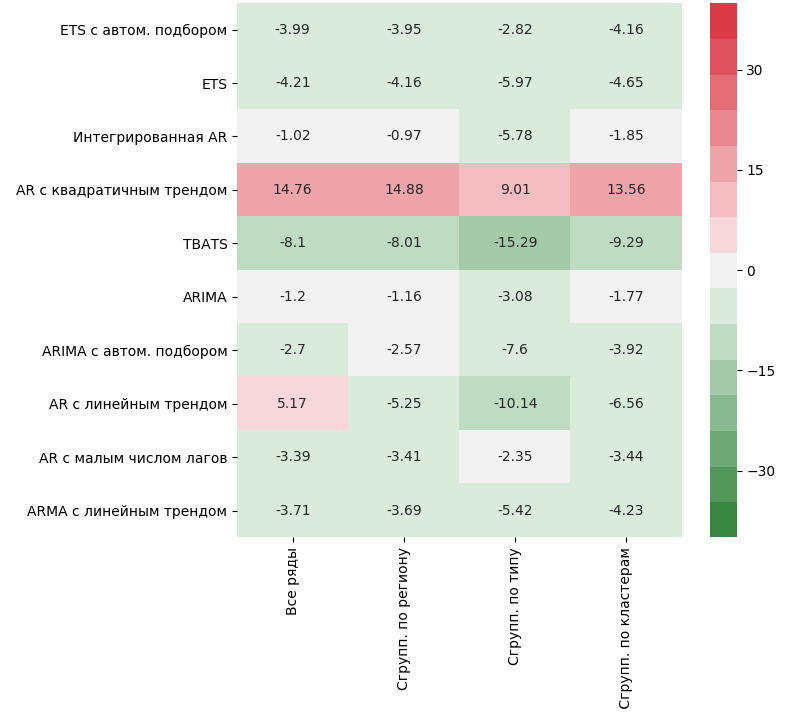
\includegraphics[width=1\linewidth]{screenshot019}}
	\end{minipage}
\end{figure}
\newpage



\thispagestyle{empty}

Выпускная квалификационная работа выполнена мной совершенно самостоятельно. Все использованные в работе материалы и концепции из опубликованной научной литературы и других источников имеют ссылки на них.

\vspace{2ex}

 Объем работы  \rule{2em}{0.5pt} листа(ов).

\vspace{2ex}

 Объем приложений \rule{2em}{0.5pt} листа(ов).

\vspace{4ex}

\noindent << \rule{1em}{0.5pt} >> \rule{5em}{0.5pt} 20 \rule{1.4em}{0.5pt} г. 

\vspace{4ex}



\noindent \rule{11em}{0.5pt} 
\hspace{8em} / Касьянова Ксения Алексеевна /

\hspace{0.5cm} \footnotesize (подпись)


%\hfill\makebox[6em]{\hfill\footnotesize (подпись) \hfill }


\end{document}
